\documentclass[a4paper]{article}
\usepackage[T1,T2A]{fontenc}
\usepackage[utf8]{inputenc}
\usepackage[english,russian]{babel}
\usepackage{booktabs}
\usepackage{color,colortbl}
%\usepackage{amsmath}
%\usepackage{amsfonts}
%\usepackage{amssymb}
%\usepackage{makeidx}
\usepackage{listings}
\usepackage{graphicx}
\usepackage{rotating}
\definecolor{green}{RGB}{45,140,31}
\definecolor{darkishgreen}{RGB}{39,203,22}
\definecolor{LightCyan}{rgb}{0.88,1,1}
\definecolor{Gray}{gray}{0.9}
\definecolor{lightRed}{RGB}{230,170,150}
\definecolor{modRed}{RGB}{230,82,90}
\definecolor{strongRed}{RGB}{230,6,6}

\lstset{ %
  language=java,                % Язык программирования
  %numbers=left,                   % С какой стороны нумеровать
  extendedchars=\true,
  %numberstyle=tinycolor{gray},     % Стиль который будет использоваться для нумерации строк
  %stepnumber=2,                   % Шаг между линиями. Если 1, то будет пронумерована каждая строка
  %numbersep=5pt,
  %backgroundcolor=color{white},      % Цвет подложки. Вы должны добавить пакет color - usepackage{color}
  showspaces=false,
  showstringspaces=false,
  showtabs=false,
  %frame=single,                    % Добавить рамку
  %rulecolor=color{black},
  tabsize=4,                       % Tab - 2 пробела
  breaklines=true,                 % Автоматический перенос строк
  breakatwhitespace=true,          % Переносить строки по словам
  title=lstname,                   % Показать название подгружаемого файла
  keywordstyle=\color{green},          % Стиль ключевых слов
  %commentstyle=color{dkgreen},       % Стиль комментариев
  %stringstyle=color{mauve}          % Стиль литералов
}

\usepackage[english,russian]{babel}

\title{
\textbf{Технология программирования}

}
\author{Романцов Григорий Дмитриевич}
\date{}

\begin{document}

\maketitle
\newpage
\tableofcontents
\newpage
\section{Введение}

\section{Отладка ПО}

Отладка —  это  процесс  определения  и  устранения  причиношибок.  Этим  она  отличается  от  тестирования,  направленного на обнаружение ошибок. В
некоторых проектах отладказанимает  до  50\%  общего  времени  разработки. Многие  программисты считают отладку самым трудным аспектом программирования.

\subsection{Общие вопросы отладки}

Грейс Хоппер  (Grace  Hopper),  контр --- адмирал  ВМС  США  и  один  из  авторов  языка  COBOL,  утверждала,  что  слово  «bug»  появилось  в  программированиив о  времена  первого  крупного  цифрового  компьютера  —  Mark  I  (IEEE,  1992).  Разбираясь  с  причинами  неисправности компьютера,  программисты  нашли  в  нем крупного  мотылька,  замкнувшего  какую-то  цепь,  и  с  тех  пор  вину  за  все  компьютерные  проблемы  стали  сваливать  на  насекомых.  Вне  программирования  слово «bug»  уходит  корнями  по  крайней  мере  во  времена  Томаса  Эдисона,  который  использовал  его  уже  в  1878  году  (Tenner,  1997)

Однако  на  самом  деле  программные  дефекты  —  не  организмы,  проникающие  в код. Это ошибки, допущенные программистами,  а  результаты  ошибок могут привести к различным последствиям (от увольнения программиста до масштабной катастрофы)

\subsubsection{Отладка и качество ПО}

Отладка,  сама  по  себе  не  служит  для  повышения  качества  ПО — это способ диагностики дефектов. О качестве нужно заботиться с самого начала  работы  над  программой.  Лучший  способ  создания  качественной  программызаключается  в  тщательной  выработке  требований,  грамотном  проектировании  и применении  высококачественных  методик  кодирования.  Отладка  —  это  средство для  крайних  случаев.

\subsubsection{Различия в эффективности отладки}

Зачем  вообще  обсуждать  отладку?  Разве  не  все  программисты  умеют  отлаживать программы?

Увы, не все. Исследования показали, что опытным программистам для нахождения  тех  же  ошибок  требовалось  примерно  в  20  раз  меньше  времени, чем неопытным. Более того, некоторые программисты находят больше дефектов  и  исправляют  их  грамотнее.  Вот  результаты  классического  исследования,  в  котором  профессиональных  программистов,  обладающих  минимум  4-летним  опытом,  попросили  отладить  программу  с  12  дефектами. Три  самых  лучших  в  отладке  программиста  смогли  найти  дефекты  примерно  в  3  раза  быстрее  и  внесли  в  код  примерно  в  2,5  раза  меньше  дефектов,  чем  три  худших.  Самый  лучший  программист  обнаружил  вседефекты  и  не  внес  во  время  их  исправления  новых.  Самый  худший  не  нашел  4  из 12  дефектов,  а  при  исправлении  8  обнаруженных  дефектов  внес  в  код  11  новых. Но ставить точку рано. После первого раунда отладки в коде самых быстрых программистов все еще остались 3,7 дефекта, а в коде самых медленных — 9,4 дефекта.  Ни  одна  из  групп  не  довела  отладку  до  конца.

Эти  данные  не  только  сообщают  нам  кое-что  об  отладке,  нои  подтверждают  Главный  Закон  Контроля  Качества  ПО:  повышение  качества  программы  снижает  затраты  на  ее  разработку.  Лучшие  программисты  обнаружили  больше  дефектовза меньшее время и исправили их более корректно. Нет нуждывыбирать  между  качеством,  стоимостью  и  быстротой  —  они  идут  рука  об  руку.

\subsubsection{Дефекты как возможности обучения}

О  чем  говорит  наличие  дефекта?  Ну,  если  исходить  из  того,  что  наличие  дефектов  в  программе  нежелательно,  это  говорит  о  том,  что  вы  не  полностью  понимаете  программу.  Это  тревожит.  Всетаки,  если  вы  написали  программу,  она  должна делать то, что вам нужно. Если вы не до конца понимаете свои указания компилятору, еще чуть --- чуть, и вы просто начнете пробовать все, что придет в голову, покачтото не сработает, т. е. начнете программировать методом проб и ошибок. А раз так,  дефекты  неизбежны.  Вам  не  нужно  учиться  исправлять  дефекты  —  вам  нужно  знать,  как  их  избегать.

Однако  люди  несовершенны,  и  даже  прекрасные  программисты  иногда  допускают  промахи.  В  таких  случаях  ошибки  предоставляют  отличные  возможности  узнать  много  нового.  Например,  вы  можете  сделать  все,  что  описано  ниже.

\noindent{\bfИзучить  программу,  над  которой  работаете} Наличие  дефекта  указываетна то, что вы должны лучше изучить программу, потому что, если б вы уже отлично  ее  знали,  в  ней  не  было  бы  дефектов.  Вы  уже  исправили  бы  их.

\noindent{\bfИзучить собственные ошибки} Все дефекты вашей программы  лежат  на  вашей  совести.  Не  каждый  день  у  вас  появляется  такая  прекрасная  возможность  лучше  узнать  собственные недостатки, и грех ее не использовать. Обнаружив ошибку,  спросите  себя,  как  и  почему  вы  допустили  ее.  Каквы могли найти ее быстрее? Как ее можно было предотвратить? Содержит ли код другие подобные ошибки? Можно ли исправить  их  до  того,  как  они  приведут  к  проблемам?

\noindent{\bfИзучить качество своего кода с точки зрения кого-то, кому придется читать его} Чтобы найти дефект, вы должны прочитать свой код. Это дает вам прекрасную возможность критически оценить его качество. Легко ли его читать? Какего  можно  улучшить?  Используйте  полученные  знания  для  рефакторинга  имеющегося  кода  или  для  улучшения  кода,  который  вы  будете  писать  позднее.

\noindent{\bfИзучить  используемые  способы  решения  проблем} Чувствуете  ли  вы  уверенность,  обдумывая  свой  подход  к  отладке?  Работает  ли  он?  Быстро  ли  вы  находите дефекты?  Может,  ваш  подход  к  отладке  неэффективен?  Чувствуете  ли  вы  тоску  и огорчение?  Не  отлаживаете  ли  вы  программу,  опираясь  на  случайные  предположения?  Нужно  ли  как-то  улучшить  процесс  отладки?  Если  учесть  объем  времени,  уходящего на отладку во многих проектах, анализ вашего способа отладки определенно не  будет  пустой  тратой  времени.  Трата  некоторого  времени  на  анализ  и  изменение процесса отладки может оказаться самым эффективным способом сокращенияобщего  времени  разработки  программы.

\noindent{\bfИзучить используемые способы исправления дефектов} Кроме способа поиска  дефектов,  вы  можете  изучить  и  свой  способ  их  исправления.  Вносите  ли  вымаксимально  простые  исправления,  используя  операторы  goto  и  частные  случаи,устраняющие  симптомы,  но  не  проблему?  Или  вы  вносите  системные  исправления,  точно  определяя  и  устраняя  причины  проблем? Вышесказанное  позволяет  сделать  вывод,  что  отладка  обеспечивает  программистам  крайне  благоприятные  возможности  для  самосовершенствования.  Именно отладка  является  перекрестком  всех  дорог  конструирования:  удобочитаемости,качества  проекта  и  кода  и  т.  д.  Именно  на  этапе  отладки  окупается  создание  хорошего  кода,  особенно  если  его  качество  редко  заставляет  прибегать  к  отладке.

\subsubsection{Неэффективный подход}

{\bfПоиск  дефектов,  основанный  на  гадании} Для  нахождения дефекта разбросайте по программе случайным образом  команды  печати  и  изучите  выходные  данные.  Если  при  помощи  команд  печати  найти  дефект  не  получается,  попробуйте  изменить  тот  или  иной  фрагмент—  может,  что  и  сработает.  Не  сохраняйте  первоначальный  вариант  программы  ине регистрируйте внесенные изменения. Если вы точно не знаете, что делает программа,  программирование  становится  более  увлекательным.  Запаситесь  колой  иледенцами,  потому  что  вам  придется  провести  перед  монитором  всю  ночь.

\noindent{\bfТщательный анализ проблемы — пустая трата времени} Скорее всего проблема  тривиальна,  и  ее  не  нужно  полностью  понимать,  чтобы  исправить.  Достаточно  ее  просто  найти.Исправление  ошибок  самым  очевидным  образомОбычно  можно  простоустранить  специфические  симптомы  проблемы,  а  не  тратить  время  на  внесениекрупного  амбициозного  исправления,  которое  может  затронуть  всю  программу.Вот  прекрасный  пример:
\begin{lstlisting}[caption=][h]
x = Compute( y )
if ( y = 17 )
    x = $25.15  — если y = 17, метод Compute() не работает; мы это исправляем
\end{lstlisting}

Зачем  анализировать  метод  Compute()  в  поисках  причин  непонятной  проблемы  созначением 17,  если  можно  просто  написать  частный  случай  в  очевидном  месте?

\subsection{Поиск дефекта}

Отладка  включает  поиск  дефекта  и  его  исправление.  Поиск  дефекта  и  его  понимание  обычно  составляют  90\%  работы.К счастью, существуют более эффективный подход к отладке, чем гадание.

Допустим,  вам  нужно  раскрыть  тайну  убийства.  Что  оказалось  бы  интереснее:обойти дома всех жителей района, проверяя их алиби, или найти несколько улики,  опираясь  на  них,  установить  убийцу?  Большинство  людей  предпочло  бы  второй  вариант,  поэтому  вполне  логично,  что  и  у  программистов  большей  популярностью  пользуется  интеллектуальный  подход  к  отладке.  Лучшие  программисты,отлаживающие  программы  в  двадцать  раз  быстрее,  чем  их  менее  квалифицированные коллеги, не гадают, как исправить дефекты. Они используют научный метод ---  основательный  процесс  анализа  и  доказательства.

\subsubsection{Научный метод отладки}

Классический  научный  метод  включает  следующие  этапы
\begin{enumerate}
  \item Сбор  данных  при  помощи  повторяющихся  экспериментов.
  \item Формулирование  гипотезы,  объясняющей  релевантные  данные.
  \item Разработка  эксперимента,  призванного  подтвердить  или  опровергнуть  гипотезу.
  \item Подтверждение  или  опровержение  гипотезы.
  \item Повторение  процесса  в  случае  надобности
\end{enumerate}

Научный  метод  имеет  много  аналогов,  используемых  при  отладке.  Нижеописан  эффективный  метод  поиска  дефекта.

\begin{enumerate}
  \item Стабилизация  ошибки.
  \item Определение  источника  ошибки.
        \begin{enumerate}
          \item Сбор  данных,  приводящих  к  дефекту.
          \item Анализ собранных данных и формулирование гипотезы, объясняющей дефект.
          \item Определение  способа  подтверждения  или  опровержения  гипотезы,  основанного  или  на  тестировании  программы,  или  на  изучении  кода.
          \item Подтверждение  или  опровержение  гипотезы  при  помощи  процедуры,определенной  в  п. 2(c).
        \end{enumerate}
  \item Исправление  дефекта.
  \item Тестирование  исправления.
  \item Поиск  похожих  ошибок.
\end{enumerate}

Первый  этап  этого  процесса  аналогичен  первому  этапу  научного  метода  в  томсмысле,  что  оба  они  основаны  на  повторяемости.  Диагностика  дефекта  облегчается,  если  его  стабилизировать,  т. е.  обеспечить  его  надежное  возникновение.Второй  этап  основан  на  этапах  научного  метода.  Вы  собираете  тестовые  данные,приводящие  к  проявлению  дефекта,  анализируете  эти  данные  и  формулируетегипотезу  об  источнике  ошибки.  Затем  вы  проектируете  тест  или  инспекцию  иоцениваете  гипотезу,  после  чего  празднуете  успех  (если  гипотеза  подтверждается)  или  начинаете  поиск  источника  ошибки  сначала.  Подтвердив  гипотезу,  выисправляете  дефект,  тестируете  исправление  и  ищете  в  коде  похожие  ошибки.Рассмотрим  все  эти  этапы  на  примере.  Допустим,  вы  столкнулись  с  несистематической  ошибкой  в  программе,  которая  работает  с  базой  данных  о  сотрудниках.Программа  должна  печатать  список  сотрудников  в  алфавитном  порядке  и  суммыподоходного  налога,  вычитаемые  из  зарплаты  каждого  сотрудника,  но  при  запуске  программы  выводится:

\begin{tabular}{lr}
Александ Александрович & 20,324 \\
Гарри Поттер               &   10,666 \\
Михаил Милый           &  100,788 \\
Мария-Тереза Михельсон           &   88,889 \\
Сендвич Сладкий      &   40,000 \\
Ярило Яркий           &   70,860 \\
\end{tabular}

Как  видите,  список  содержит  ошибку:  записи  сотрудников  Мария-Тереза Михельсон, и Михаил Милый  выведены  в  неверном  порядке.

\subsubsection{Стабилизация ошибки}

Если  дефект  проявляется  не  всегда,  его  почти  невозможно  диагностировать.  Перевод не систематического дефекта в разряд предсказуемых — один из самых сложных  аспектов  отладки.

Непредсказуемые ошибки обычно связаны с инициализацией,  расчетом  времени  или  зависшими  указателями.  Еслисумма  иногда  вычисляется  правильно,  а  иногда  неправильно, это, вероятно, объясняется тем, что одна из переменныхне  инициализируется  и  просто  получает  в  большинстве  случаев  нулевое  значение.  Если  вы  столкнулись  со  странной  непредсказуемой  проблемой  при  работе  суказателями,  почти  наверняка  ее  причина  —  неинициализированный  указательили  использование  указателя  после  освобождения  соответствующей  ему  областипамяти.Стабилизация  ошибки  обычно  не  ограничивается  нахождением  теста,  приводящего  к  ошибке.  Она  предполагает  упрощение  теста  до  тех  пор,  пока  не  будет  получен  самый  простой  тест,  все  еще  приводящий  к  ошибке.  Иначе  говоря,  тестследует  сделать  таким  простым,  чтобы  изменение  любого  его  аспекта  изменяло поведение  ошибки.  Затем,  тщательно  изменяя  тест  и  наблюдая  за  поведением программы  в  контролируемых  условиях,  вы  можете  диагностировать  проблему. Если  в  вашей  организации  есть  независимая  группа  тестирования,  упрощение тестов  иногда  можно  поручить  ей,  но  в  большинстве  случаев  это  ваша  работа. Для  упрощения  теста  также  следует  использовать  научный  метод.  Допустим,  вы определили 10 факторов, комбинация которых приводит к ошибке. Сформулируйт египотезу о том, какие факторы нерелевантны для возникновения ошибки. Изменитеэти  факторы  и  выполните  тест  еще  раз.  Если  ошибка  никуда  не  исчезает,  вы  можете  упростить  тест,  исключив  эти  факторы.  Затем  вы  можете  попробовать  сделатьтест  еще  проще.  Если  ошибка  больше  не  возникает,  значит,  вы  опровергли  конкретную  гипотезу  и  получили  дополнительные  сведения  о  проблеме.  Возможно, другие  изменения  все  еще  будут  приводить  к  ошибке,  но  теперь  вы  хотя  бы  знаете одно  конкретное  изменение,  после  внесения  которого  ошибка  исчезает.

В нашем случае при первом запуске программы запись Мария-Тереза Михельсон выводитсяв  списке  после  Михаил Милый.  Однако  при  втором  запуске  записи  выводятся  вправильном  порядке:

\begin{tabular}{lr}
Александ Александрович & 20,324 \\
Гарри Поттер               &   10,666 \\
Мария-Тереза Михельсон           &   88,889 \\
Михаил Милый           &  100,788 \\
Сендвич Сладкий      &   40,000 \\
Ярило Яркий           &   70,860 \\
\end{tabular}

После  ввода  записи Ар-Истарх Аристархович  которая  появляется  в  неверной  позиции,  вывспоминаете, что запись Михаил Милый также была введена непосредственно перед отображением  некорректного  списка.  Что  необычно  в  этих  случаях,  так  это  то,что записи были введены по отдельности. Как правило, данные вводятся сразу для нескольких  сотрудников. Итак,  можно  предположить,  что  проблема  как-то  связана  с  вводом  одной  новой записи. Если это так, то при следующем запуске программы запись Ар-Истарх Аристархович должна  занять  правильное  место.  Ну-ка,  проверим:

\begin{tabular}{lr}
Александ Александрович & 20,324 \\
Ар-Истарх Аристархович  &   50,877 \\
Гарри Поттер               &   10,666 \\
Максим Малый           &   88,889 \\
Михаил Милый           &  100,788 \\
Сендвич Сладкий      &   40,000 \\
Ярило Яркий           &   70,860 \\
\end{tabular}

Правильная  сортировка  списка  соответствует  выдвинутой  гипотезе.  И  все  же  для ее  окончательного  подтверждения  следует  добавить  несколько  новых  записей  поодной  за  раз  и  посмотреть,  выводятся  ли  они  в  неверном  порядке  при  первомзапуске  программы  и  изменяется  ли  их  порядок  при  втором.

\subsubsection{Определение источника ошибки}

Определение  источника  ошибки  также  призывает  к  использованию  научногометода.  Так,  вы  могли  бы  заподозрить,  что  дефект  является  результатом  конкретной  проблемы,  такой  как  ошибка  занижения  или  завышения  на  1.  Для  проверки этой  гипотезы  вы  могли  бы  присвоить  параметру,  который  предположительно вызывает  проблему,  значение,  равное  граничному  условию,  а  также  два  значения,отличающихся  от  граничного  условия  на  1. В нашем примере причиной проблемы может быть занижение или завышение на 1  при  добавлении  одной  новой  записи,  но  не  двух  или  более.  Однако  изучение кода  не  приводит  к  нахождению  очевидной  ошибки  занижения  или  завышения на 1. Тогда вы обращаетесь к плану Б и добавляете в БД одну новую запись, чтобы увидеть,  вызовет  ли  это  проблему.  Вы  добавляете  запись  Иван Иванов  и  предполагаете,  что  она  займет  неправильное  место.  При  запуске  программы  выводится:

\begin{tabular}{lr}
Александ Александрович & 20,324 \\
Ар-Истарх Аристархович  &   50,877 \\
Гарри Поттер               &   10,666 \\
Иван Иванов           & 40,323\\
Мария-Тереза Михельсон           &   88,889 \\
Михаил Милый           &  100,788 \\
Сендвич Сладкий      &   40,000 \\
Ярило Яркий           &   70,860 \\
\end{tabular}

Список  отсортирован  правильно,  а  значит,  первая  гипотеза  ошибочна.  Добавление одного нового сотрудника не является причиной проблемы. Проблема имеетили  более  сложную,  или  совсем  другую  природу.При  более  внимательном  изучении  выходных  данных  теста  можно  заметить,  что только записи Ар-Истарх Аристархович и Мария-Тереза Михельсон включают дефисы. Сразу же послеввода  запись Ар-Истарх Аристархович  занимала  неверное  положение,  но  с  записью  Мария-Тереза Михельсон  было  в  порядке,  ведь  так?  Хотя  распечатки  результатов  самого  первого  запуска программы у вас нет, вы помните, что вас смутило место записи Михаил Милый, но  она  располагалась  по  соседству  с Мария-Тереза.  Возможно,  ошибочным  было положение  записи  Мария-тереза,  а  не  Михаил. Вы  выдвигаете  новую  гипотезу:  причина  проблемы  связана  с  фамилиями,  содержащими  дефисы,  а  не  с  фамилиями,  которые  вводятся  по  одной. Но как это объясняет тот факт, что проблема возникает только при вводе записи? Вы  изучаете  код  и  замечаете,  что  в  программе  используются  два  разных  метода сортировки:  один  вызывается  при  вводе  записи,  а  второй  —  при  ее  сохранении.Более  тщательный  анализ  первого  метода  показывает,  что  он  и  не  должен  сортировать  список  полностью.  Вставляя  новую  запись,  он  лишь  приблизительноопределяет  ее  положение  для  ускорения  сортировки,  которую  выполняет  второйметод.  Так  что  проблема  в  том,  что  данные  печатаются  до  их  сортировки.  Фамилии,  содержащие  дефисы,  располагаются  в  неправильном  порядке  изза  того,  чтометод  примерной  сортировки  не  обрабатывает  подобные  тонкости.  Теперь  выможете  выдвинуть  еще  более  точную  гипотезу:  фамилии,  содержащие  знаки  пунктуации,  правильно  сортируются  только  во  время  сохранения.

Далее  вы  подтверждаете  эту  гипотезу  при  помощи  дополнительных  тестов.

\subsubsection{Советы по поиску причин дефектов}

После стабилизации ошибки и уточнения вызывающих ее условий поиск ее можетбыть  как  тривиальным,  так  и  трудным:  это  зависит  от  того,  насколько  хорошо  написан  код.  Если  найти  причину  дефекта  не  удается,  возможно,  это  обусловленонизким  качеством  кода.  Каким  бы  неприятным  ни  был  такой  вывод,  ничего  не  поделаешь:  это  правда.  В  подобной  ситуации  вам  помогут  следующие  советы.

{\bfФормулируя  гипотезу,  используйте  все  имеющиеся  данные} Выдвигая  гипотезу  об  источнике  дефекта,  постарайтесь  учесть  как  можно  больше  данных.В нашем примере вы могли бы обратить внимание на неверное место записи Ар-Истарх  и  предположить,  что  неверно  сортируются  все  фамилии,  начинающиеся на букву «А». Гипотеза неудачна: она не объясняет неправильное место записи Михаил И Мария-Тереза  и  правильную  сортировку  записей  при  втором  запуске  программы.  Если  данные  не  соответствуют  гипотезе,  не  игнорируйте  их  —  подумайте,почему  они  ей  не  соответствуют,  и  сформулируйте  новую  гипотезу. Вторая  наша  гипотеза,  согласно  которой  причина  проблемы  связана  с  фамилиями,  содержащими  дефисы,  а  не  с  вводом  фамилий  по  одной,  также  первоначально  не  объясняла  правильную  сортировку  фамилий  при  повторном  выполнении программы.  Однако  она  привела  нас  к  более  точной  гипотезе,  оказавшейся  верной.  Если  первая  гипотеза  не  объясняет  все  данные,  ничего  страшного  —  улучшайте  ее,  пока  не  достигнете  этой  цели.

{\bfДетализируйте тесты, приводящие к ошибке} Если вы не можете найти источник  ошибки,  попробуйте  уточнить  уже  имеющиеся  тесты.  Возможно,  изменение  какого-нибудь  из  параметров  в  более  широком  диапазоне  или  концентрация на  одном  из  параметров  позволит  сдвинуть  отладку  с  мертвой  точки.

{\bfПроверяйте код при помощи блочных тестов} Как правило,  в  небольших  фрагментах  кода  дефекты  искать  легче,чем  в  крупных  интегрированных  программах.  Используйте для изолированного тестирования фрагментов кода блочные  тесты.

{\bfИспользуйте  разные  инструменты} На  рынке  имеются  многочисленные  инструменты, облегчающие отладку: интерактивные отладчики, строгие компиляторы,инструменты  проверки  памяти,  утилиты  проверки  синтаксиса  и  т.  д.  Правильныйинструмент способен сделать трудную работу простой. Мне вспоминается случай,когда одна неуловимая ошибка заставляла одну часть программы перезаписыватьпамять  другой  части.  Традиционные  методики  отладки  не  помогли  в  поискахошибки:  программист  не  мог  определить,  какой  именно  фрагмент  перезаписывал  память.  Тогда  он  установил  точку  прерывания  на  конкретный  адрес  памяти.Когда  программа  выполнила  запись  по  этому  адресу,  отладчик  прервал  ее  выполнение,  и  виновный  код  был  обнаружен.Это пример проблемы, которую трудно диагностировать аналитически, но довольнолегко  с  помощью  правильного  инструмента.

{\bfВоспроизведите  ошибку  несколькими  способами} Иногда  полезную  информацию  можно  получить,  выполнив  тест,  похожий  на  тесты,  приводящие  к  ошибке, но не идентичный им. Можете рассматривать этот подход как триангулирование  дефекта.  Воспроизведя  дефект  несколькими  способами,  вы  точнее  определите  его  источник. Воспроизведение ошибки разными способами помогает диагностировать причину ошибки. Как только вы решили, что причина дефекта ясна, выполнитетест,  который  сам  не  должен  вызывать  ошибку,  но  напоминает  тесты,  приводящие  к  ошибке.  Если  ошибка  при  этом  все  же  возникает,  значит,  вы  еще  не  полностью  поняли  проблему.  Причиной  ошибки  часто  становится  комбинация  факторов,  поэтому  попытка  диагностировать  проблему  при  помощи  только  одного  теста  часто  не  приводит  к  обнаружению  корня  проблемы.

\begin{figure}[h]
\center{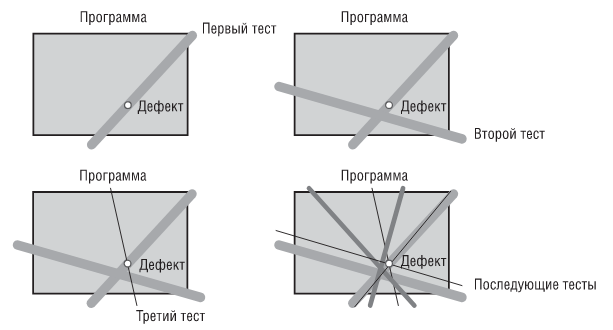
\includegraphics[width=\textwidth]{o1.png}}
\end{figure}

{\bfГенерируйте больше данных для формулирования большего числа гипотез} Выберите  тесты,  отличающиеся  от  тестов,  результаты  которых  уже  известны. Выполните  их,  чтобы  получить  дополнительные  данные  и  использовать  их  длявыдвижения  дополнительных  гипотез.

{\bfИспользуйте  результаты  отрицательных  тестов} Предположим,  что  вывыдвинули  гипотезу  и  запустили  тест  с  целью  ее  подтверждения.  Допустим  далее,что  тест  опроверг  гипотезу,  так  что  причина  ошибки  все  еще  неизвестна.  И  всеже  вы  узнали  нечто  полезное:  одно  из  ваших  предположений  о  причинах  дефекта  ошибочно.  Это  сужает  область  поиска  и  уменьшает  число  оставшихся  гипотез.

{\bfИспользуйте  «мозговой  штурм»  для  построения  нескольких  гипотез}Неостанавливайтесь  на  первой  пришедшей  в  голову  гипотезе,  а  попробуйте  выдвинуть  несколько  гипотез.  Не  анализируйте  их  сразу  —  просто  придумайте  за  несколько  минут  максимальное  число  гипотез.  Затем  рассмотрите  их  по  очереди  иподумайте  о  тестах,  которые  могут  их  доказать  или  опровергнуть.  Это  упражнение  помогает  сдвинуть  отладку  с  мертвой  точки,  обусловленной  слишком  сильной  концентрацией  на  одной  линии  рассуждения.

{\bfСоставьте  список  подходов,  которые  стоит  попробовать} Иногда  программисты  не  могут  найти  ошибку  по  той  причине,  что  слишком  долго  следовали  по  пути,  ведущему  в  тупик. Составьте  список  подходов,  которые  стоит  попробовать,  и,  если  один  из  них  не  работает,  переходите  к  следующему.

{\bfСократите  подозрительную  область  кода} Вместо  тестирования  всей  программы, всего класса или метода протестируйте сначала меньший фрагмент кода.Используйте  для  нахождения  ошибочного  фрагмента  команды  печати,  записьинформации  в  журнал  или  трассировку.Есть  и  более  эффективный  способ  сужения  подозрительной  области  кода:  систематически  удаляйте  части  программы  и  смотрите,  возникает  ли  ошибка.  Еслиошибка  исчезла,  ищите  ее  в  удаленной  части.  Если  ошибка  попрежнему  возникает,  дефектный  код  все  еще  присутствует  в  программе.Вместо  удаления  случайных  фрагментов  руководствуйтесь  принципом  «разделяйи  властвуй».  Используйте  алгоритм  двоичного  поиска.  Попробуйте  удалить  в  первый  раз  примерно  половину  кода.  Определите  половину,  содержащую  дефект,  иразделите  ее.  Снова  определите  дефектную  половину  и  снова  разделите  ее  пополам.  Продолжайте,  пока  дефект  не  будет  найден.Если  программа  содержит  много  небольших  методов,  можете  убирать  фрагментыкода,  просто  комментируя  вызовы  методов.  В  противном  случае  можете  блокировать  фрагменты  кода  при  помощи  комментариев  или  директив  препроцессора.Работая с отладчиком, удалять фрагменты кода не обязательно. Вместо этого можнозадать  точки  прерывания.  Если  отладчик  позволяет  пропускать  вызовы  методов,попробуйте найти дефектный код, пропуская выполнение определенных методови  наблюдая,  исчезает  ли  после  этого  ошибка.  Этот  процесс  во  многом  похож  надействительное  удаление  фрагментов  программы.

{\bfС  подозрением  относитесь  к  классам  и  методам,  которые содержали дефекты ранее} Классы, которые были дефектными раньше, более подвержены ошибкам. Новыедефекты  чаще  обнаруживаются  в  классах,  с  которыми  ираньше  были  связаны  проблемы,  а  не  в  классах,  которыебыли  безошибочными.  Проанализируйте  подверженныеошибкам  классы  и  методы  еще  раз.

{\bfПроверьте  код,  который  был  изменен  недавно} Если  у  вас  появилась  новаянепростая ошибка, она скорее всего содержится в фрагменте, который был изменен  недавно.  Ее  источником  может  быть  как  абсолютно  новый  код,  так  и  измененный  старый.  Если  вы  не  можете  найти  дефект,  запустите  старую  версию  программы  и  проверьте,  возникает  ли  ошибка.  Если  нет,  ошибка  содержится  в  новомкоде  или  объясняется  взаимодействием  с  новым  кодом.  Изучите  различия  междустарой  и  новой  версиями.  Посмотрите  в  журнале  системы  управления  версиями,какой  код  был  изменен  недавно.  Если  это  невозможно,  используйте  для  сравнения  старого  работоспособного  и  нового  дефектного  кода  другой  инструмент.

{\bfРасширьте подозрительный фрагмент кода}Сосредоточиться на небольшомфрагменте  кода  легко,  но  это  принесет  пользу,  только  если  дефект  навернякасодержится  в  этом  фрагменте.  Если  дефект  не  удается  найти  в  конкретной  области  кода,  рассмотрите  вероятность  того,  что  его  в  ней  нет.  Расширьте  подозрительную  область  кода  и  проанализируйте  ее,  применив  описанную  выше  методику  двоичного  поиска.

{\bfВыполняйте интеграцию инкрементно} Отладка будетлегкой,  если  вы  будете  добавлять  элементы  в  систему  по  одному за раз. Если после добавления нового элемента возниклановая  ошибка,  удалите  его  и  протестируйте  отдельно.

\subsubsection{Стандартыне техники отладки}

\begin{enumerate}
  \item Отладка с помощью дебаггера.

        (софтварного, железячного или удалённого дебагера) с пошаговой отладкой, просмотром состояний (переменных, стека, памяти, регистров, тредов и т.п.) в требуемых точках исполнения программы.
  \item Отладка с помощью зрительного анализа кода.

        поиск причин возникновения дефекта с помощью анализа исходного кода программы, проблемного контента, конфигурации, состояния базы данных и т.п.
  \item Отладка с помощью прототипирования.

        Проверка функций (модулей, библиотек, и т.п.) в изоляции с помощью небольших примеров кода (прототипов). Прототип легче отлаживать, чем целевую систему. Если проблема воспроизводиться с помощью прототипа, отладка упрощается. Unit тестирование в этом смысле более эффективный метод отладки, поскольку unit test-ы выполняются автоматически и «накапливаются» для будущего реюза, а прототипы редко становятся частью системы.
  \item Профилирование кода.

        (если необходима оптимизация производительности) — разновидность логирования кода, хотя часто выполняется с использованием специализированных инструментальных средств (профилировщиков). Этот метод отладки позволяет получить профиль исполнения программы — сколько и какая функция, строчка кода, модуль, и т.п. отнимают процессорного времени, и таким образом найти узкие места.
  \item Выполнение кода в другой среде.

        (операционной системе, эмуляторе, симуляторе) — основная идея в том, что если нет инструментальных средств на целевой платформе, то можно спортировать код на другую платформу, где они есть. Также можно изначально писать кросс-платформенный код системы или какой-то её части, и таким образом, при необходимости практически без портирования отлаживать код на другой платформе.
  \item Отладка с помощью RPC.

         (remote procedure call)  — применимо в основном для встроенного программирования. Суть метода в возможности вызвать любую функцию (модуль и т.п.) передавая аргументы и получая результаты исполнения удалённо с одного хоста на другом вместо того, чтобы тратить время на компиляцию или обновление софта на удалённом хосте (или железке). Существуют множество готовых фреймворков (правда в основном платных), которые инструментируют код и позволяют вызывать любые функции кода через USB или IP соединения.
  \item Отладка путем анализа документации и файлов проекта.

        дизайна, требований или ограничений модулей (программных или аппаратных) — применимо в основном для сложных и крупных проектов. Основная идея понять по имеющейся документации допустимо ли поведение, происходящее в дефекте. Например, поддерживается ли сложная комбинация одновременно работающих фич. Если  поведение не поддерживается, то необходимо просто программно закрыть use-case, вместо того, чтобы пытаться глубоко анализировать код или пытаться найти root-cause в third-party компонентах.
  \item Отладка трансляцией кода.

        сложный алгоритм пишется или прототипируется на одном языке программирования (возможно медленном или интерпретируемом) с наличием всех доступных инструментальных средств (дебагера и т.п.), а потом исходный код отлаженного алгоритма транслируется в ручную или автоматически в другой язык программирования (целевой системы), для которого отсутствуют необходимые инструментальный средства. При таком подходе отладится можно на практически любом удобном для себя языке программирования, а потом заново странслировать программу на целевой язык программирования. Возможны и другие варианты, например,  дисассемблерование с целью более низкоуровневого понимания, что происходит при выполнении программы. Т.е. анализируется некий промежуточный вариант кода, который в некоторых ситуациях легче отладить или понять.
  \item Отладка разработкой интерпретатора.

        это не только метод отладки, но и паттерн проектирования. Этот метод используется, когда модуль требует частых изменений (из-за плавающих требований или поддержки большого количества фич, железок и т.п.), а время построения приложения очень большое. Для ускорения процесса и гибкости пишется небольшой интерпретатор кода с наличием управляющих конструкций if, циклов, goto. При наличии такого интерпретатора разработчик сравнительно не сложно создаёт скрипты, которые  можно быстрее исправить и отладить. Как упрощённый вариант такого способа отладки, например, использование дебажных флагов в коде, которые конфигурируют код и позволяют проверить разные варианты исполнения кода сделав лишь один build.
\end{enumerate}

\subsubsection{Итоги}

Отладка  —  это  тот  этап  разработки  программы,  от  которого  зависит  возможность ее выпуска. Конечно, лучше всего вообще избегать ошибок, используя другиеметодики,  описанные  в  этой  книге.  Однако  потратить  время  на  улучшение  навыков  отладки  все  же  стоит,  потому  что  эффективность  отладки,  выполняемойлучшими  и  худшими  программистами,  различается  минимум  в  10  раз.

Систематичный  подход  к  поиску  и  исправлению  ошибок  —  непременное  условие  успешности  отладки.  Организуйте  отладку  так,  чтобы  каждый  тест  приближал  вас  к  цели.  Используйте  Научный  Метод  Отладки.

Прежде  чем  приступать  к  исправлению  программы,  поймите  суть  проблемы.Случайные предположения о причинах ошибок и случайные исправления только  ухудшат  программу.

Установите  в  настройках  компилятора  самый  строгий  уровень  диагностики  иустраняйте причины всех ошибок и предупреждений. Как вы исправите неуловимые  ошибки,  если  будете  игнорировать  явные?

Инструменты  отладки  значительно  облегчают  разработку  ПО.  Найдите  их  ииспользуйте,  но  не  забывайте,  что  у  вас  есть  еще  и  голова.

\section{Архитектура ПО}

Правильная архитектура экономит очень много сил, времени и денег. А нередко вообще определяет то, выживет ваш проект или нет. И даже если речь идет всего лишь о «построении табуретки» все равно вначале очень полезно ее спроектировать. Сложность, как правило, растет гораздо быстрее размеров программы. И если не позаботиться об этом заранее, то довольно быстро наступает момент, когда ты перестаешь ее контролировать.

\subsection{Критерии хорошей архитектуры}

Вообще говоря, не существует общепринятого термина «архитектура программного обеспечения». Тем не менее, когда дело касается практики, то для большинства разработчиков и так понятно какой код является хорошим, а какой плохим. Хорошая архитектура это прежде всего выгодная архитектура, делающая процесс разработки и сопровождения программы более простым и эффективным. Программу с хорошей архитектурой легче расширять и изменять, а также тестировать, отлаживать и понимать. То есть, на самом деле можно сформулировать список вполне разумных и универсальных критериев:

\noindent\textbf{Эффективность системы.} В первую очередь программа, конечно же, должна решать поставленные задачи и хорошо выполнять свои функции, причем в различных условиях. Сюда можно отнести такие характеристики, как надежность, безопасность, производительность, способность справляться с увеличением нагрузки (масштабируемость) и т.п.

\noindent\textbf{Гибкость системы.} Любое приложение приходится менять со временем — изменяются требования, добавляются новые. Чем быстрее и удобнее можно внести изменения в существующий функционал, чем меньше проблем и ошибок это вызовет — тем гибче и конкурентоспособнее система. Поэтому в процессе разработки старайтесь оценивать то, что получается, на предмет того, как вам это потом, возможно, придется менять. Спросите у себя: «А что будет, если текущее архитектурное решение окажется неверным?», «Какое количество кода подвергнется при этом изменениям?». Изменение одного фрагмента системы не должно влиять на ее другие фрагменты. По возможности, архитектурные решения не должны «вырубаться в камне», и последствия архитектурных ошибок должны быть в разумной степени ограничены. "Хорошая архитектура позволяет ОТКЛАДЫВАТЬ принятие ключевых решений" (Боб Мартин) и минимизирует «цену» ошибок.

\noindent\textbf{Расширяемость системы.} Возможность добавлять в систему новые сущности и функции, не нарушая ее основной структуры. На начальном этапе в систему имеет смысл закладывать лишь основной и самый необходимый функционал (принцип YAGNI — you ain’t gonna need it, «Вам это не понадобится») Но при этом архитектура должна позволять легко наращивать дополнительный функционал по мере необходимости. Причем так, чтобы внесение наиболее вероятных изменений требовало наименьших усилии.

Требование, чтобы архитектура системы обладала гибкостью и расширяемостью (то есть была способна к изменениям и эволюции) является настолько важным, что оно даже сформулировано в виде отдельного принципа — «Принципа открытости/закрытости» (Open-Closed Principle — второй из пяти принципов SOLID): Программные сущности (классы, модули, функции и т.п.) должны быть открытыми для расширения, но закрытыми для модификации.

Иными словами: Должна быть возможность расширить/изменить поведение системы без изменения/переписывания уже существующих частей системы.

Это означает, что приложение следует проектировать так, чтобы изменение его поведения и добавление новой функциональности достигалось бы за счет написания нового кода (расширения), и при этом не приходилось бы менять уже существующий код. В таком случае появление новых требований не повлечет за собой модификацию существующей логики, а сможет быть реализовано прежде всего за счет ее расширения. Именно этот принцип является основой «плагинной архитектуры» (Plugin Architecture). О том, за счет каких техник это может быть достигнуто, будет рассказано дальше.

\noindent\textbf{Масштабируемость процесса разработки.} Возможность сократить срок разработки за счёт добавления к проекту новых людей. Архитектура должна позволять распараллелить процесс разработки, так чтобы множество людей могли работать над программой одновременно.

\noindent\textbf{Тестируемость.} Код, который легче тестировать, будет содержать меньше ошибок и надежнее работать. Но тесты не только улучшают качество кода. Многие разработчики приходят к выводу, что требование «хорошей тестируемости» является также направляющей силой, автоматически ведущей к хорошему дизайну, и одновременно одним из важнейших критериев, позволяющих оценить его качество: "Используйте принцип «тестируемости» класса в качестве «лакмусовой бумажки» хорошего дизайна класса. Даже если вы не напишите ни строчки тестового кода, ответ на этот вопрос в 90\% случаев поможет понять, насколько все «хорошо» или «плохо» с его дизайном" (Идеальная архитектура).

Существует целая методология разработки программ на основе тестов, которая так и называется — Разработка через тестирование (Test-Driven Development, TDD).

\noindent\textbf{Возможность повторного использования.} Систему желательно проектировать так, чтобы ее фрагменты можно было повторно использовать в других системах.

\noindent\textbf{Хорошо структурированный, читаемый и понятный код.} Сопровождаемость. Над программой, как правило, работает множество людей — одни уходят, приходят новые. После написания сопровождать программу тоже, как правило, приходится людям, не участвовавшем в ее разработке. Поэтому хорошая архитектура должна давать возможность относительно легко и быстро разобраться в системе новым людям. Проект должен быть хорошо структурирован, не содержать дублирования, иметь хорошо оформленный код и желательно документацию. И по возможности в системе лучше применять стандартные, общепринятые решения привычные для программистов. Чем экзотичнее система, тем сложнее ее понять другим (Принцип наименьшего удивления — Principle of least astonishment. Обычно, он используется в отношении пользовательского интерфейса, но применим и к написанию кода).

\noindentНу и для полноты критерии плохого дизайна:
\begin{enumerate}
\item Его тяжело изменить, поскольку любое изменение влияет на слишком большое количество других частей системы. (Жесткость, Rigidity).
\item При внесении изменений неожиданно ломаются другие части системы. (Хрупкость, Fragility).
\item Код тяжело использовать повторно в другом приложении, поскольку его слишком тяжело «выпутать» из текущего приложения. (Неподвижность, Immobility).
\end{enumerate}

\subsection{Модульная архитектура. Декомпозиция как основа}

\begin{figure}[h]
\center{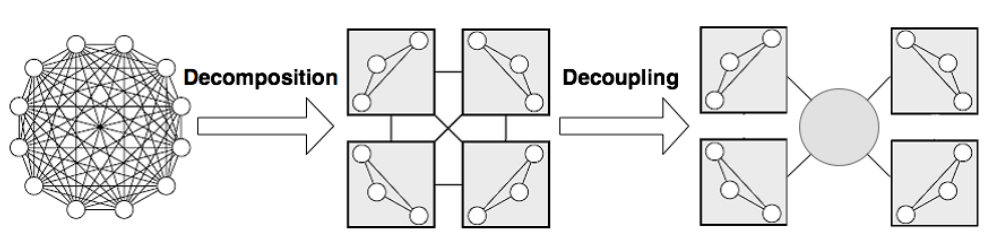
\includegraphics[width=\textwidth]{a1.png}}
\end{figure}


Не смотря на разнообразие критериев, все же главной при разработке больших систем считается задача снижения сложности. А для снижения сложности ничего, кроме деления на части, пока не придумано. Иногда это называют принципом «разделяй и властвуй» (divide et impera), но по сути речь идет об иерархической декомпозиции. Сложная система должна строится из небольшого количества более простых подсистем, каждая из которых, в свою очередь, строится из частей меньшего размера, и т.д., до тех пор, пока самые небольшие части не будут достаточно просты для непосредственного понимания и создания.

Удача заключается в том, что данное решение является не только единственно известным, но и универсальным. Помимо снижения сложности, оно одновременно обеспечивает гибкость системы, дает хорошие возможности для масштабирования, а также позволяет повышать устойчивость за счет дублирования критически важных частей.

Соответственно, когда речь идет о построении архитектуры программы, создании ее структуры, под этим, главным образом, подразумевается декомпозиция программы на подсистемы (функциональные модули, сервисы, слои, подпрограммы) и организация их взаимодействия друг с другом и внешним миром. Причем, чем более независимы подсистемы, тем безопаснее сосредоточиться на разработке каждой из них в отдельности в конкретный момент времени и при этом не заботиться обо всех остальных частях.

В этом случае программа из «спагетти-кода» превращается в конструктор, состоящий из набора модулей/подпрограмм, взаимодействующих друг с другом по хорошо определенным и простым правилам, что собственно и позволяет контролировать ее сложность, а также дает возможность получить все те преимущества, которые обычно соотносятся с понятием хорошая архитектура:
\begin{itemize}
    \item \textbf{Масштабируемость (Scalability)}
    возможность расширять систему и увеличивать ее производительность, за счет добавления новых модулей.
    \item \textbf{Ремонтопригодность (Maintainability)}
    изменение одного модуля не требует изменения других модулей
    \item \textbf{Заменимость модулей (Swappability)}
    модуль легко заменить на другой
    \item \textbf{Возможность тестирования (Unit Testing)}
    модуль можно отсоединить от всех остальных и протестировать / починить
    \item \textbf{Переиспользование (Reusability)}
    модуль может быть переиспользован в других программах и другом окружении
    \item \textbf{Сопровождаемость (Maintenance)}
    разбитую на модули программу легче понимать и сопровождать
\end{itemize}

Можно сказать, что в разбиении сложной проблемы на простые фрагменты и заключается цель всех методик проектирования. А термином «архитектура», в большинстве случаев, просто обозначают результат такого деления, плюс "некие конструктивные решения, которые после их принятия с трудом поддаются изменению" (Мартин Фаулер «Архитектура корпоративных программных приложений»). Поэтому большинство определений в той или иной форме сводятся к следующему:

"Архитектура идентифицирует главные компоненты системы и способы их взаимодействия. Также это выбор таких решений, которые интерпретируются как основополагающие и не подлежащие изменению в будущем."

"Архитектура — это организация системы, воплощенная в ее компонентах, их отношениях между собой и с окружением.
Система — это набор компонентов, объединенных для выполнения определенной функции."

Таким образом, хорошая архитектура это, прежде всего, модульная/блочная архитектура. Чтобы получить хорошую архитектуру надо знать, как правильно делать декомпозицию системы. А значит, необходимо понимать — какая декомпозиция считается «правильной» и каким образом ее лучше проводить?

\subsection{«Правильная» декомпозиция}

\subsubsection{Иерархическая}

Не стоит сходу рубить приложение на сотни классов. Как уже говорилось, декомпозицию надо проводить иерархически — сначала систему разбивают на крупные функциональные модули/подсистемы, описывающие ее работу в самом общем виде. Затем, полученные модули, анализируются более детально и, в свою очередь, делятся на под-модули либо на объекты.

Перед тем как выделять объекты разделите систему на основные смысловые блоки хотя бы мысленно. Для небольших приложений двух уровней иерархии часто оказывается вполне достаточно — система вначале делится на подсистемы/пакеты, а пакеты делятся на классы.

\begin{figure}[h]
\center{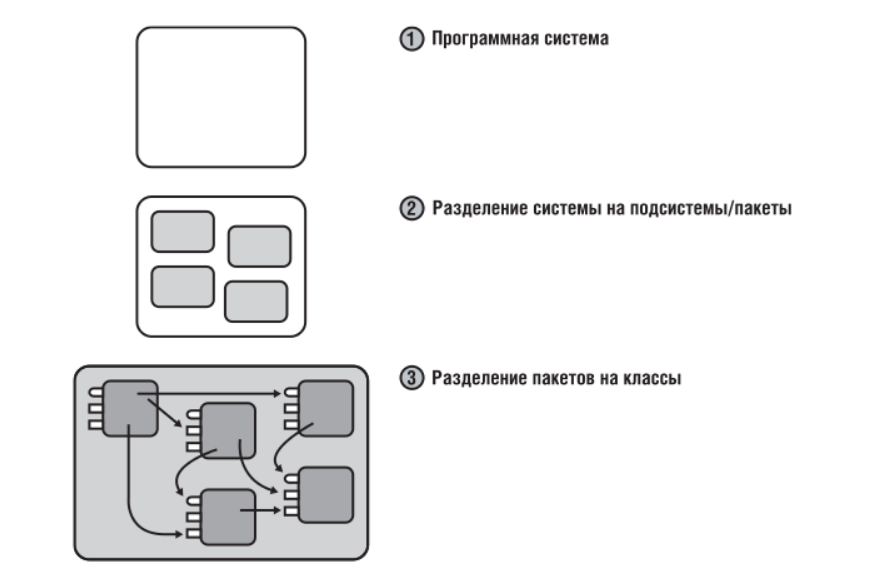
\includegraphics[width=\textwidth]{a2.png}}
\end{figure}

Эта мысль, при всей своей очевидности, не так банальна как кажется. Например, в чем заключается суть такого распространенного «архитектурного шаблона» как Модель-Вид-Контроллер (MVC)? Всего навсего в отделении представления от бизнес-логики, то есть в том, что любое пользовательское приложение вначале делится на два модуля — один из которых отвечает за реализацию собственно самой бизнес логики (Модель), а второй — за взаимодействие с пользователем (Пользовательский Интерфейс или Представление). Затем, для того чтобы эти модули могли разрабатываться независимо, связь между ними ослабляется с помощью паттерна «Наблюдатель» (подробно о способах ослабления связей будет рассказано дальше) и мы фактически получаем один из самых мощных и востребованных «шаблонов», которые используются в настоящее время.

Типичными модулями первого уровня (полученными в результате первого деления системы на наиболее крупные составные части) как раз и являются — «бизнес-логика», «пользовательский интерфейс», «доступ к БД», «связь с конкретным оборудованием или ОС».

Для обозримости на каждом иерархическом уровне рекомендуют выделять от 2 до 7 модулей.

\subsubsection{Функциональная}

Деление на модули/подсистемы лучше всего производить исходя из тех задач, которые решает система. Основная задача разбивается на составляющие ее подзадачи, которые могут решаться/выполняться независимо друг от друга. Каждый модуль должен отвечать за решение какой-то подзадачи и выполнять соответствующую ей функцию. Помимо функционального назначения модуль характеризуется также набором данных, необходимых ему для выполнения его функции, то есть:

\textit{Модуль = Функция + Данные, необходимые для ее выполнения.}

Причем желательно, чтобы свою функцию модуль мог выполнить самостоятельно, без помощи остальных модулей, лишь на основе своих входящих данных.

Модуль — это не произвольный кусок кода, а отдельная функционально осмысленная и законченная программная единица (подпрограмма), которая обеспечивает решение некоторой задачи и в идеале может работать самостоятельно или в другом окружении и быть переиспользуемой. Модуль должен быть некой "целостностью, способной к относительной самостоятельности в поведении и развитии" (Кристофер Александер).

Таким образом, грамотная декомпозиция основывается, прежде всего, на анализе функций системы и необходимых для выполнения этих функций данных.

\subsubsection{High Cohesion + Low Coupling}

Самым же главным критерием качества декомпозиции является то, насколько модули сфокусированы на решение своих задач и независимы. Обычно это формулируют следующим образом: "Модули, полученные в результате декомпозиции, должны быть максимально сопряженны внутри (high internal cohesion) и минимально связанны друг с другом (low external coupling)."

\begin{itemize}
\item \textbf{High Cohesion}, высокая сопряженность или «сплоченность» внутри модуля, говорит о том, модуль сфокусирован на решении одной узкой проблемы, а не занимается выполнением разнородных функций или несвязанных между собой обязанностей. (Сопряженность — cohesion, характеризует степень, в которой задачи, выполняемые модулем, связаны друг с другом )

Следствием High Cohesion является принцип единственной ответственности (Single Responsibility Principle — первый из пяти принципов SOLID), согласно которому любой объект/модуль должен иметь лишь одну обязанность и соответственно не должно быть больше одной причины для его изменения.

\item \textbf{Low Coupling}, слабая связанность, означает что модули, на которые разбивается система, должны быть, по возможности, независимы или слабо связанны друг с другом. Они должны иметь возможность взаимодействовать, но при этом как можно меньше знать друг о друге (принцип минимального знания).

Это значит, что при правильном проектировании, при изменении одного модуля, не придется править другие или эти изменения будут минимальными. Чем слабее связанность, тем легче писать/понимать/расширять/чинить программу.
\end{itemize}

Считается, что хорошо спроектированные модули должны обладать следующими свойствами:
\begin{itemize}
    \item {\bfфункциональная целостность и завершенность} — каждый модуль реализует одну функцию, но реализует хорошо и полностью; модуль самостоятельно (без помощи дополнительных средств) выполняет полный набор операций для реализации своей функции.
    \item {\bfодин вход и один выход} — на входе программный модуль получает определенный набор исходных данных, выполняет содержательную обработку и возвращает один набор результатных данных, т.е. реализуется стандартный принцип IPO — вход–процесс–выход;
    \item {\bfлогическая независимость} — результат работы программного модуля зависит только от исходных данных, но не зависит от работы других модулей;
    слабые информационные связи с другими модулями — обмен информацией между модулями должен быть по возможности минимизирован.
\end{itemize}

Грамотная декомпозиция — это своего рода искусство и гигантская проблема для многих программистов. Простота тут очень обманчива, а ошибки обходятся очень дорого. Если выделенные модули оказываются сильно сцеплены друг с другом, если их не удается разрабатывать независимо или не ясно за какую конкретно функцию каждый из них отвечает, то стоит задуматься а правильно ли вообще производится деление. Должно быть понятно, какую роль выполняет каждый модуль. Самый же надежный критерий того, что декомпозиция делается правильно, это если модули получаются самостоятельными и ценными сами по себе подпрограммами, которые могут быть использованы в отрыве от всего остального приложения (а значит, могут быть переиспользуемы).

Делая декомпозицию системы желательно проверять ее качество задавая себе вопросы: "Какую функцию выполняет каждый модуль?", “Насколько модули легко тестировать?”, “Возможно ли использовать модули самостоятельно или в другом окружении?”, “Как сильно изменения в одном модуле отразятся на остальных?”

В первую очередь следует, конечно же, стремиться к тому, чтобы модули были предельно автономны. Как и было сказано, это является ключевым параметром правильной декомпозиции. Поэтому проводить ее нужно таким образом, чтобы модули изначально слабо зависели друг от друга. Но кроме того, имеется ряд специальных техник и шаблонов, позволяющих затем дополнительно минимизировать и ослабить связи между подсистемами. Например, в случае MVC для этой цели использовался шаблон «Наблюдатель», но возможны и другие решения. Можно сказать, что техники для уменьшения связанности, как раз и составляют основной «инструментарий архитектора». Только необходимо понимать, что речь идет о всех подсистемах и ослаблять связанность нужно на всех уровнях иерархии, то есть не только между классам, но также и между модулями на каждом иерархическом уровне.

\subsection{Как ослаблять связанность между модулями}

\subsubsection{Интерфейсы. Фасад}

Главным, что позволяет уменьшать связанность системы, являются конечно же Интерфейсы (и стоящий за ними принцип Инкапсуляция + Абстракция + Полиморфизм):

\begin{itemize}
\item Модули должны быть друг для друга "черными ящиками" (инкапсуляция). Это означает, что один модуль не должен «лезть» внутрь другого модуля и что либо знать о его внутренней структуре. Объекты одной подсистемы не должны обращаться напрямую к объектам другой подсистемы
\item Модули/подсистемы должны взаимодействовать друг с другом лишь посредством интерфейсов (то есть, абстракций, не зависящих от деталей реализации) Соответственно каждый модуль должен иметь четко определенный интерфейс или интерфейсы для взаимодействия с другими модулями.
\end{itemize}

Принцип «черного ящика» (инкапсуляция) позволяет рассматривать структуру каждой подсистемы независимо от других подсистем. Модуль, представляющий собой черный ящик, можно относительно свободно менять. Проблемы могут возникнуть лишь на стыке разных модулей (или модуля и окружения). И вот это взаимодействие нужно описывать в максимально общей (абстрактной) форме — в форме интерфейса. В этом случае код будет работать одинаково с любой реализацией, соответствующей контракту интерфейса. Собственно именно эта возможность работать с различными реализациями (модулями или объектами) через унифицированный интерфейс и называется полиморфизмом. Полиморфизм это вовсе не переопределение методов, как иногда ошибочно полагают, а прежде всего — взаимозаменяемость модулей/объектов с одинаковым интерфейсом, или «один интерфейс, множество реализаций». Для реализации полиморфизма механизм наследования совсем не нужен. Это важно понимать, поскольку наследования вообще, по возможности, следует избегать.

Благодаря интерфейсам и полиморфизму, как раз и достигается возможность модифицировать и расширять код, без изменения того, что уже написано (Open-Closed Principle). До тех пор, пока взаимодействие модулей описано исключительно в виде интерфейсов, и не завязано на конкретные реализации, мы имеем возможность абсолютно «безболезненно» для системы заменить один модуль на любой другой, реализующий тот же самый интерфейс, а также добавить новый и тем самым расширить функциональность. Это как в конструкторе или «плагинной архитектуре» (plugin architecture) — интерфейс служит своего рода коннектором, куда может быть подключен любой модуль с подходящим разъемом. Гибкость конструктора обеспечивается тем, что мы можем просто заменить одни модули/«детали» на другие, с такими же разъемами (с тем же интерфейсом), а также добавить сколько угодно новых деталей (при этом уже существующие детали никак не изменяются и не переделываются).

Интерфейсы позволяют строить систему более высокого уровня, рассматривая каждую подсистему как единое целое и игнорируя ее внутреннее устройство. Они дают возможность модулям взаимодействовать и при этом ничего не знать о внутренней структуре друг друга, тем самым в полной мере реализуя принцип минимального знания, являющейся основой слабой связанности. Причем, чем в более общей/абстрактной форме определены интерфейсы и чем меньше ограничений они накладывают на взаимодействие, тем гибче система. Отсюда фактически следует еще один из принципов SOLID — Принцип разделения интерфейса (Interface Segregation Principle), который выступает против «толстых интерфейсов» и говорит, что большие, объемные интерфейсы надо разбивать на более маленькие и специфические, чтобы клиенты маленьких интерфейсов (зависящие модули) знали только о методах, которые необходимы им в работе. Формулируется он следующим образом: "Клиенты не должны зависеть от методов (знать о методах), которые они не используют" или “Много специализированных интерфейсов лучше, чем один универсальный”.

Итак, когда взаимодействие и зависимости модулей описываются лишь с помощью интерфейсов, те есть абстракций, без использования знаний об их внутреннем устройстве и структуре, то фактически тем самым реализуется инкапсуляция, плюс мы имеем возможность расширять/изменять поведения системы за счет добавления и использования различных реализаций, то есть за счет полиморфизма. Из этого следует, что концепция интерфейсов включает в себя и в некотором смысле обобщает почти все основные принципы ООП — Инкапсуляцию, Абстракцию, Полиморфизм. Но тут возникает один вопрос. Когда проектирование идет не на уровне объектов, которые сами же и реализуют соответствующие интерфейсы, а на уровне модулей, то что является реализацией интерфейса модуля? Ответ: если говорить языком шаблонов, то как вариант, за реализацию интерфейса модуля может отвечать специальный объект — Фасад.

Фасад — это объект-интерфейс, аккумулирующий в себе высокоуровневый набор операций для работы с некоторой подсистемой, скрывающий за собой ее внутреннюю структуру и истинную сложность. Обеспечивает защиту от изменений в реализации подсистемы. Служит единой точкой входа — "вы пинаете фасад, а он знает, кого там надо пнуть в этой подсистеме, чтобы получить нужное".


Таким образом, мы получаем первый, самый важный паттерн, позволяющий использовать концепцию интерфейсов при проектировании модулей и тем самым ослаблять их связанность — «Фасад». Помимо этого «Фасад» вообще дает возможность работать с модулями точно также как с обычными объектами и применять при проектировании модулей все те полезные принципы и техники, которые используются при проектирования классов.

\begin{figure}[h]
\center{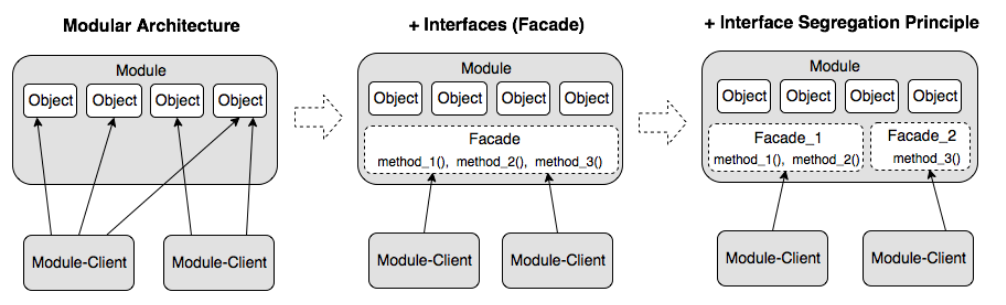
\includegraphics[width=\textwidth]{a3.png}}
\end{figure}

\subsubsection{Dependency Inversion. Корректное создание и получение зависимостей}

Формально, требование, чтобы модули не содержали ссылок на конкретные реализации, а все зависимости и взаимодействие между ними строились исключительно на основе абстракций, то есть интерфейсов, выражается принципом Инвертирования зависимостей (Dependency Inversion — последний из пяти принципов SOLID):
\begin{itemize}
\item Модули верхнего уровня не должны зависеть от модулей нижнего уровня. И те, и другие должны зависеть от абстракций.
\item Абстракции не должны зависеть от деталей. Реализация должна зависеть от абстракции.
\end{itemize}

У этого принципа не самая очевидная формулировка, но суть его, как и было сказано, выражается правилом: «Все зависимости должны быть в виде интерфейсов».
Не смотря на свою фундаментальность и кажущуюся простоту это правило нарушается, пожалуй, чаще всего. А именно, каждый раз, когда в коде программы/модуля мы используем оператор new и создаем новый объект конкретного типа, то тем самым вместо зависимости от интерфейса образуется зависимость от реализации.

Понятно, что этого нельзя избежать и объекты где-то должны создаваться. Но, по крайней мере, нужно свести к минимуму количество мест, где это делается и в которых явно указываются классы, а также локализовать и изолировать такие места, чтобы они не были разбросаны по всему коду программы.

В каком-то смысле такое решение следует Принципу единственного выбора (Single Choice Principle), который говорит: "всякий раз, когда система программного обеспечения должна поддерживать множество альтернатив, их полный список должен быть известен только одному модулю системы". В этом случае, если в будущем придется добавить новые варианты (или новые реализации, как в рассматриваемом нами случае создания новых объектов), то достаточно будет произвести обновление только того модуля, в котором содержится эта информация, а все остальные модули останутся незатронутыми и смогут продолжать свою работу как обычно.

Ну а теперь разберем подробнее, как это делается на практике и каким образом модули могут корректно создавать и получать свои «зависимости», не нарушая принципа Dependency Inversion.

Итак, при проектировании модуля должны быть определены следующие ключевые вещи:
\begin{enumerate}
        \item что модуль делает, какую функцию выполняет
    \item что модулю нужно от его окружения, то есть с какими объектами/модулями ему придется иметь дело и
      \item как он это будет получать
\end{enumerate}

Крайне важно то, как модуль получает ссылки на объекты, которые он использует в своей работе. И тут возможны следующие варианты:

\noindent1. Модуль сам создает объекты необходимые ему для работы.

Но, как и было сказано, модуль не может это сделать напрямую — для создания необходимо вызвать конструктор конкретного типа, и в результате модуль будет зависеть не от интерфейса, а от конкретной реализации. Решить проблему в данном случае позволяет шаблон Фабричный Метод (Factory Method).

"Суть заключается в том, что вместо непосредственного инстанцирования объекта через new, мы предоставляем классу-клиенту некоторый интерфейс для создания объектов. Поскольку такой интерфейс при правильном дизайне всегда может быть переопределён, мы получаем определённую гибкость при использовании низкоуровневых модулей в модулях высокого уровня".

В случаях, когда нужно создавать группы или семейства взаимосвязанных объектов, вместо Фабричного Метода используется Абстрактная Фабрика (Abstract factory).

\noindent2. Модуль берет необходимые объекты у того, у кого они уже есть (обычно это некоторый, известный всем репозиторий, в котором уже лежит все, что только может понадобиться для работы программы).
Этот подход реализуется шаблоном Локатор Сервисов (Service Locator), основная идея которого заключается в том, что в программе имеется объект, знающий, как получить все зависимости (сервисы), которые могут потребоваться.

Главное отличие от фабрик в том, что Service Locator не создаёт объекты, а фактически уже содержит в себе инстанцированные объекты (или знает где/как их получить, а если и создает, то только один раз при первом обращении). Фабрика при каждом обращении создает новый объект, который вы получаете в полную собственность и можете делать с ним что хотите. Локатор же сервисов выдает ссылки на одни и те же, уже существующие объекты. Поэтому с объектами, выданными Service Locator, нужно быть очень осторожным, так как одновременно с вами ими может пользоваться кто-то еще.

Объекты в Service Locator могут быть добавлены напрямую, через конфигурационный файл, да и вообще любым удобным программисту способом. Сам Service Locator может быть статическим классом с набором статических методов, синглетоном или интерфейсом и передаваться требуемым классам через конструктор или метод.

Вообще говоря, Service Locator иногда называют антипаттерном и не рекомендуют использовать (главным образом потому, что он создает неявные связности и дает лишь видимость хорошего дизайна).

\noindent3. Модуль вообще не заботиться о «добывании» зависимостей. Он лишь определяет, что ему нужно для работы, а все необходимые зависимости ему поставляются («впрыскиваются») из вне кем-то другим.

Это так и называется — Внедрение Зависимостей (Dependency Injection). Обычно требуемые зависимости передаются либо в качестве параметров конструктора (Constructor Injection), либо через методы класса (Setter injection).

Такой подход инвертирует процесс создания зависимости — вместо самого модуля создание зависимостей контролирует кто-то извне. Модуль из активного элемента, становится пассивным — не он делает, а для него делают. Такое изменение направления действия называется Инверсия Контроля (Inversion of Control), или Принцип Голливуда — «Не звоните нам, мы сами вам позвоним».

Это самое гибкое решение, дающее модулям наибольшую автономность. Можно сказать, что только оно в полной мере реализует «Принцип единственной ответственности» — модуль должен быть полностью сфокусирован на том, чтобы хорошо выполнять свою функцию и не заботиться ни о чем другом. Обеспечение его всем необходимым для работы это отдельная задача, которой должен заниматься соответствующий «специалист» (обычно управлением зависимостями и их внедрениями занимается некий контейнер — IoC-контейнер).

По сути, здесь все как в жизни: в хорошо организованной компании программисты программируют, а столы, компьютеры и все необходимое им для работы покупает и обеспечивает кладовщик. Или, если использовать метафору программы как конструктора — модуль не должен думать о проводах, сборкой конструктора занимается кто-то другой, а не сами детали.

Не будет преувеличением сказать, что использование интерфейсов для описания зависимостей между модулями (Dependency Inversion) + корректное создание и внедрение этих зависимостей (прежде всего Dependency Injection) являются центральными/базовыми техниками для снижения связанности. Они служат тем фундаментом, на котором вообще держится слабая связанность кода, его гибкость, устойчивость к изменениям, переиспользование, и без которого все остальные техники имеют мало смысла. Но, если с фундаментом все в порядке, то знание дополнительных приемов может быть очень даже полезным.

\subsubsection{Замена прямых зависимостей на обмен сообщениями}

Иногда модулю нужно всего лишь известить других о том, что в нем произошли какие-то события/изменения и ему не важно, что с этой информацией будет происходить потом. В этом случае модулям вовсе нет необходимости «знать друг о друге», то есть содержать прямые ссылки и взаимодействовать непосредственно, а достаточно всего лишь обмениваться сообщениями (messages) или событиями (events).

Связь модулей через обмен сообщениями является гораздо более слабой, чем прямая зависимость и реализуется она чаще всего с помощью следующих шаблонов:
\begin{itemize}
\item Наблюдатель (Observer). Применяется в случае зависимости «один-ко-многим», когда множество модулей зависят от состояния одного — основного. Использует механизм рассылки, который заключается в том, что основной модуль просто осуществляет рассылку одинаковых сообщений всем своим подписчикам, а модули, заинтересованные в этой информации, реализуют интерфейс «подписчика» и подписываются на рассылку. Находит широкое применение в системах с пользовательским интерфейсом, позволяя ядру приложения (модели) оставаться независимым и при этом информировать связанные с ним интерфейсы о том что произошли какие-то изменения и нужно обновиться.

Организация взаимодействия посредством рассылки сообщений имеет дополнительный «бонус» — необязательность существования «подписчиков» на «опубликованные» (т.е. рассылаемые) сообщения. Качественно спроектированная подобная система допускает добавление/удаление модулей в любое время.

\item Посредник (Mediator). Применяется, когда между модулями имеется зависимость «многие ко многим. Медиатор выступает в качестве посредника в общении между модулями, действуя как центр связи и избавляет модули от необходимости явно ссылаться друг на друга. В результате взаимодействие модулей друг с другом («все со всеми») заменяется взаимодействием модулей лишь с посредником («один со всеми»). Говорят, что посредник инкапсулирует взаимодействие между множеством модулей.

\begin{figure}[h]
\center{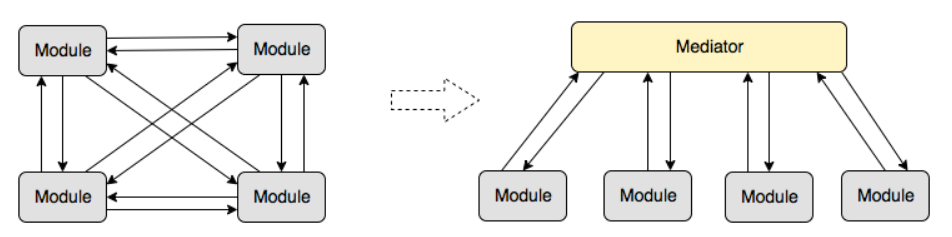
\includegraphics[width=\textwidth]{a4.png}}
\end{figure}

Типичный пример — контроль трафика в аэропорту. Все сообщения, исходящие от самолетов, поступают в башню управления диспетчеру, вместо того, чтобы пересылаться между самолетами напрямую. А диспетчер уже принимает решения о том, какие самолеты могут взлетать или садиться, и в свою очередь отправляет самолетам соответствующие сообщения.

\end{itemize}

\subsubsection{Замена прямых зависимостей на синхронизацию через общее ядро}

Данный подход обобщает и развивает идею заложенную в шаблоне «Посредник». Когда в системе присутствует большое количество модулей, их прямое взаимодействие друг с другом становится слишком сложным. Поэтому имеет смысл взаимодействие «все со всеми» заменить на взаимодействие «один со всеми». Для этого вводится некий обобщенный посредник, это может быть общее ядро приложения, хранилище или шина данных, а все остальные модули становятся независимыми друг от друга клиентами, использующими сервисы этого ядра или выполняющими обработку содержащейся там информации. Реализация этой идеи позволяет модулям-клиентам общаться друг с другом через посредника и при этом ничего друг о друге не знать.

Ядро-посредник может как знать о модулях-клиентах и управлять ими (пример — архитектура apache ), так и может быть полностью, или почти полностью, независимым и ничего о клиентах не знать. В сущности именно этот подход реализован в «шаблоне» Модель-Вид-Контроллер (MVC), где с одной Моделью (являющейся ядром приложение и общим хранилищем данных) могут взаимодействовать множество Пользовательских Интерфейсов, которые работают синхронно и при этом не знают друг о друге, а Модель не знает о них. Ничто не мешает подключить к общей модели и синхронизировать таким образом не только интерфейсы, но и другие вспомогательные модули.

Очень активно эта идея также используется при разработке игр, где независимые модули, отвечающие за графику, звук, физику, управление программой синхронизируются друг с другом через игровое ядро (модель), где хранятся все данные о состоянии игры и ее персонажах. В отличие от MVC, в играх согласование модулей с ядром (моделью) происходит не за счет шаблона «Наблюдатель», а по таймеру, что само по себе является интересным архитектурным решением весьма полезным для программ с анимацией и «бегущей» графикой.

\subsubsection{Закон Деметры (law of Demeter)}

Закон Деметры запрещает использование неявных зависимостей: "Объект A не должен иметь возможность получить непосредственный доступ к объекту C, если у объекта A есть доступ к объекту B и у объекта B есть доступ к объекту C". Java-пример.

Это означает, что все зависимости в коде должны быть «явными» — классы/модули могут использовать в работе только «свои зависимости» и не должны лезть через них к другим. Кратко этот принцип формулируют еще таким образом: "Взаимодействуй только с непосредственными друзьями, а не с друзьями друзей". Тем самым достигается меньшая связанность кода, а также большая наглядность и прозрачность его дизайна.

Закон Деметры реализует уже упоминавшийся «принцип минимального знания», являющейся основой слабой связанности и заключающийся в том, что объект/модуль должен знать как можно меньше деталей о структуре и свойствах других объектов/модулей и вообще чего угодно, включая собственные подкомпоненты. Аналогия из жизни: Если Вы хотите, чтобы собака побежала, глупо командовать ее лапами, лучше отдать команду собаке, а она уже разберётся со своими лапами сама.

\subsubsection{Композиция вместо наследования}

Одну из самых сильных связей между объектами дает наследование, поэтому, по возможности, его следует избегать и заменять композицией.

\newpage
\section{Принцыпы SOLID}

\begin{figure}[h]
\center{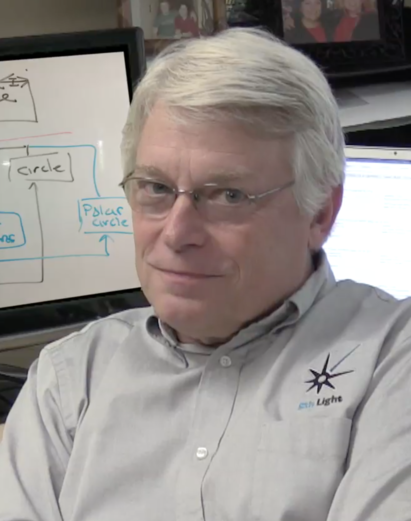
\includegraphics[scale=0.4]{uncle_bob.png}}
\end{figure}

Объектно --- ориентированное программирование принесло в разработку ПО новые подходы к проектированию приложений. В частности, ООП позволило программистам комбинировать сущности, объединённые некоей общей целью или функционалом, в отдельных классах, рассчитанных на решение самостоятельных задач и независимых от других частей приложения. Однако само по себе применение ООП не означает, что разработчик застрахован от возможности создания непонятного, запутанного кода, который тяжело поддерживать. Роберт Мартин, для того, чтобы помочь всем желающим разрабатывать качественные ООП --- приложения, разработал пять принципов объектно --- ориентированного программирования и проектирования, говоря о которых, с подачи Майкла Фэзерса, используют акроним SOLID.\@
\newline
\newline
\noindent\textbf{Что такое SOLID?}

Вот как расшифровывается акроним SOLID:\@
\begin{itemize}
    \item S:\@Single Responsibility Principle (Принцип единственной ответственности).
    \item O:\@ Open-Closed Principle (Принцип открытости-закрытости).
    \item L:\@Liskov Substitution Principle (Принцип подстановки Барбары Лисков).
    \item I:\@Interface Segregation Principle (Принцип разделения интерфейса).
    \item D:\@Dependency Inversion Principle (Принцип инверсии зависимостей).
\end{itemize}
Сейчас мы рассмотрим эти принципы на схематичных примерах. Обратите внимание на то, что главная цель примеров заключается в том, чтобы помочь читателю понять принципы SOLID, узнать, как их применять и как следовать им, проектируя приложения. \textit{Автор материала не стремился к тому, чтобы выйти на работающий код, который можно было бы использовать в реальных проектах.}

\subsection{Принцип единственной ответственности}

\textit{«Одно поручение. Всего одно.» — Локи говорит Скурджу в фильме «Тор: Рагнарёк».
Каждый класс должен решать лишь одну задачу.}

Класс должен быть ответственен лишь за что-то одно. Если класс отвечает за решение нескольких задач, его подсистемы, реализующие решение этих задач, оказываются связанными друг с другом. Изменения в одной такой подсистеме ведут к изменениям в другой.

Обратите внимание на то, что этот принцип применим не только к классам, но и к компонентам программного обеспечения в более широком смысле.

Например, рассмотрим этот код:

\begin{figure}[h]
\center{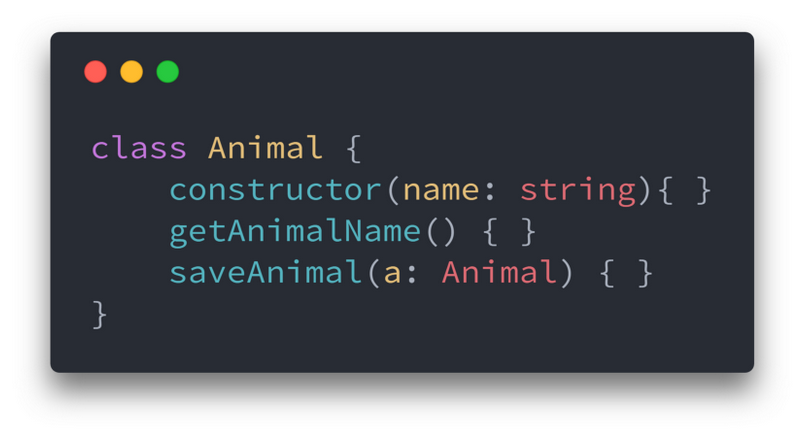
\includegraphics[width=\textwidth]{l1.png}}
\end{figure}

Класс Animal, представленный здесь, описывает какое-то животное. Этот класс нарушает принцип единственной ответственности. Как именно нарушается этот принцип?

В соответствии с принципом единственной ответственности класс должен решать лишь какую-то одну задачу. Он же решает две, занимаясь работой с хранилищем данных в методе saveAnimal и манипулируя свойствами объекта в конструкторе и в методе getAnimalName.

Как такая структура класса может привести к проблемам?

Если изменится порядок работы с хранилищем данных, используемым приложением, то придётся вносить изменения во все классы, работающие с хранилищем. Такая архитектура не отличается гибкостью, изменения одних подсистем затрагивают другие, что напоминает эффект домино.

Для того чтобы привести вышеприведённый код в соответствие с принципом единственной ответственности, создадим ещё один класс, единственной задачей которого является работа с хранилищем, в частности — сохранение в нём объектов класса Animal:

\begin{figure}[h]
\center{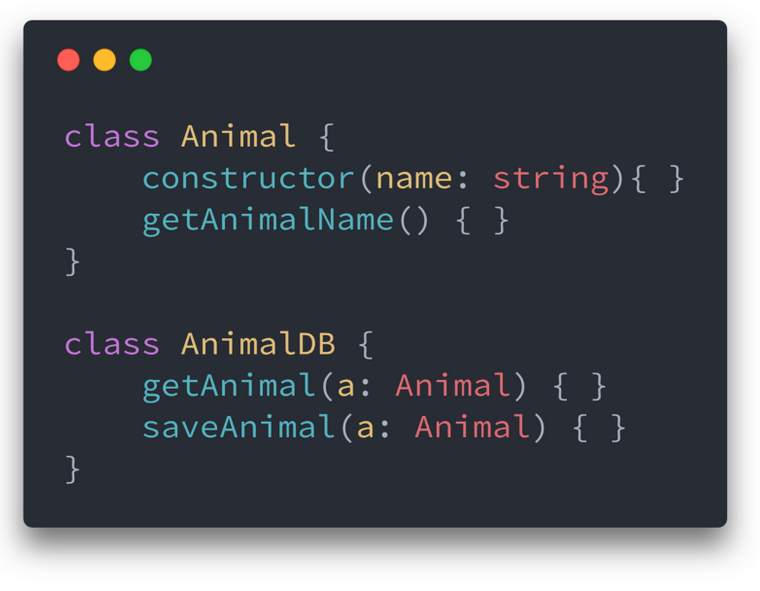
\includegraphics[width=\textwidth]{l2.png}}
\end{figure}

Вот что по этому поводу говорит Стив Фентон: «Проектируя классы, мы должны стремиться к тому, чтобы объединять родственные компоненты, то есть такие, изменения в которых происходят по одним и тем же причинам. Нам следует стараться разделять компоненты, изменения в которых вызывают различные причины».

Правильное применение принципа единственной ответственности приводит к высокой степени связности элементов внутри модуля, то есть к тому, что задачи, решаемые внутри него, хорошо соответствуют его главной цели.

\subsection{Принцип открытости-закрытости}

\textit{Программные сущности (классы, модули, функции) должны быть открыты для расширения, но не для модификации.}

Продолжим работу над классом Animal.

\begin{figure}[h]
\center{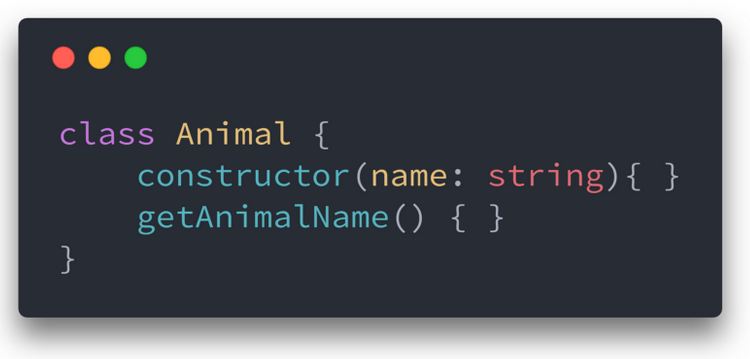
\includegraphics[scale=0.3]{l3.png}}
\end{figure}

Мы хотим перебрать список животных, каждое из которых представлено объектом класса Animal, и узнать о том, какие звуки они издают. Представим, что мы решаем эту задачу с помощью функции AnimalSounds:

\begin{figure}[h]
\center{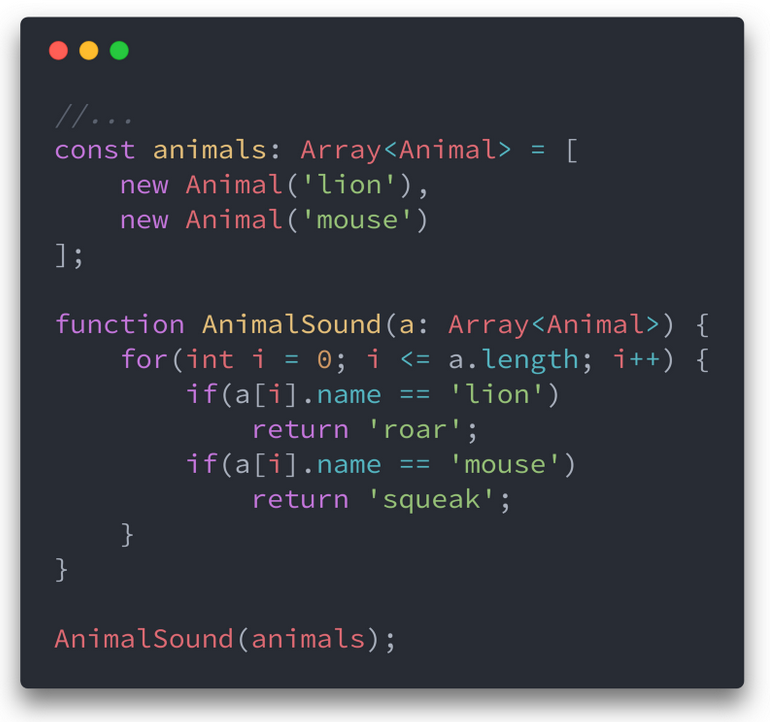
\includegraphics[scale=0.3]{l4.png}}
\end{figure}

Самая главная проблема такой архитектуры заключается в том, что функция определяет то, какой звук издаёт то или иное животное, анализируя конкретные объекты. Функция AnimalSound не соответствует принципу открытости-закрытости, так как, например, при появлении новых видов животных, нам, для того, чтобы с её помощью можно было бы узнавать звуки, издаваемые ими, придётся её изменить.

\newpage
Добавим в массив новый элемент:

\begin{figure}[h]
\center{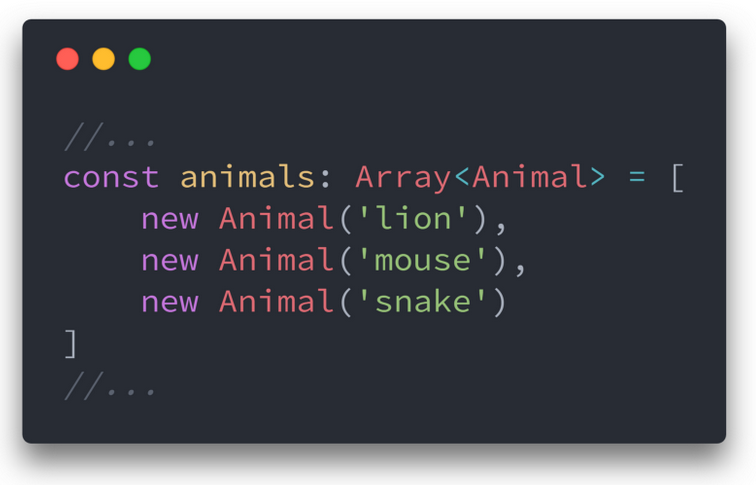
\includegraphics[scale=0.3]{l5.png}}
\end{figure}

После этого нам придётся поменять код функции AnimalSound:

\begin{figure}[h]
\center{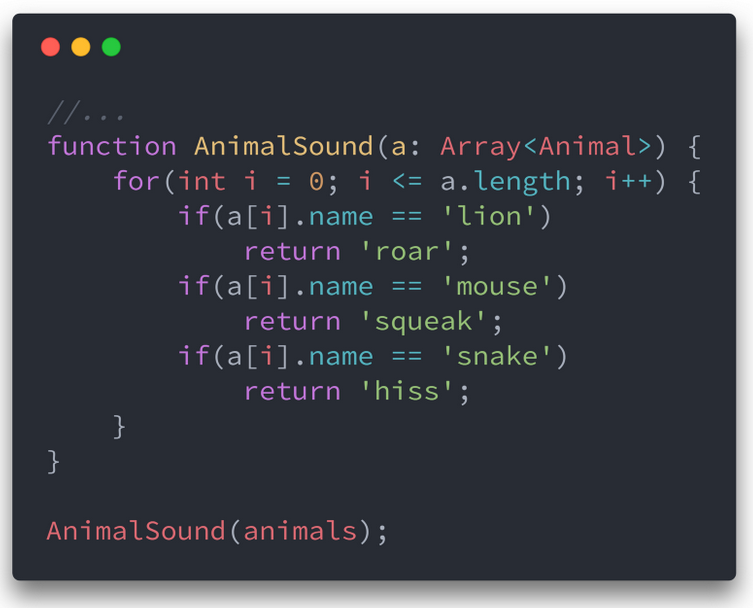
\includegraphics[scale=0.3]{l6.png}}
\end{figure}

Как видите, при добавлении в массив нового животного придётся дополнять код функции. Пример это очень простой, но если подобная архитектура используется в реальном проекте, функцию придётся постоянно расширять, добавляя в неё новые выражения if.

\newpage
Как привести функцию AnimalSound в соответствие с принципом открытости-закрытости? Например — так:

\begin{figure}[h]
\center{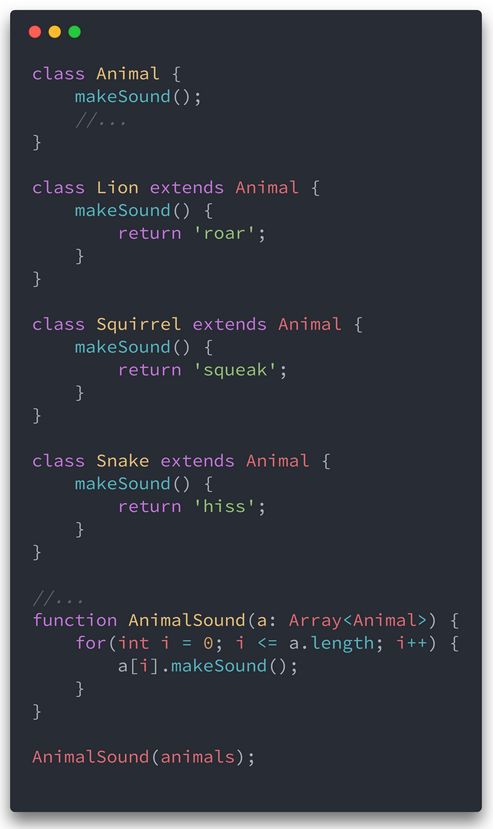
\includegraphics[scale=0.3]{l7.png}}
\end{figure}

Можно заметить, что у класса Animal теперь есть виртуальный метод makeSound. При таком подходе нужно, чтобы классы, предназначенные для описания конкретных животных, расширяли бы класс Animal и реализовывали бы этот метод.

В результате у каждого класса, описывающего животного, будет собственный метод makeSound, а при переборе массива с животными в функции AnimalSound достаточно будет вызвать этот метод для каждого элемента массива.

Если теперь добавить в массив объект, описывающий новое животное, функцию AnimalSound менять не придётся. Мы привели её в соответствие с принципом открытости-закрытости.

Рассмотрим ещё один пример.

\newpage
Представим, что у нас есть магазин. Мы даём клиентам скидку в 20\%, используя такой класс:

\begin{figure}[h]
\center{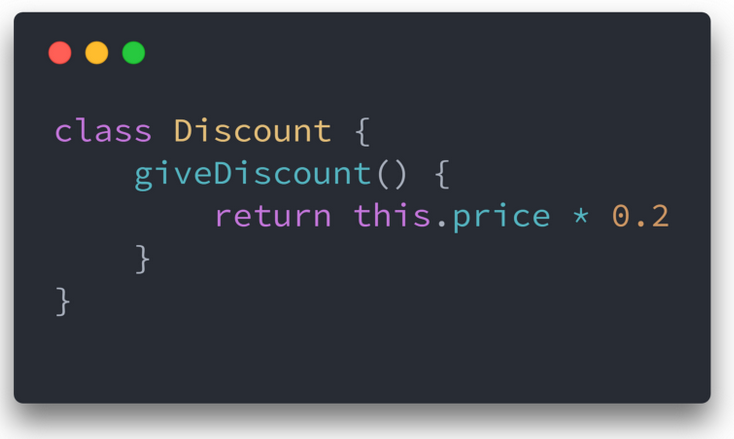
\includegraphics[scale=0.3]{l8.png}}
\end{figure}

Теперь решено разделить клиентов на две группы. Любимым (fav) клиентам даётся скидка в 20\%, а VIP-клиентам (vip) — удвоенная скидка, то есть — 40\%. Для того, чтобы реализовать эту логику, было решено модифицировать класс следующим образом:

\begin{figure}[h]
\center{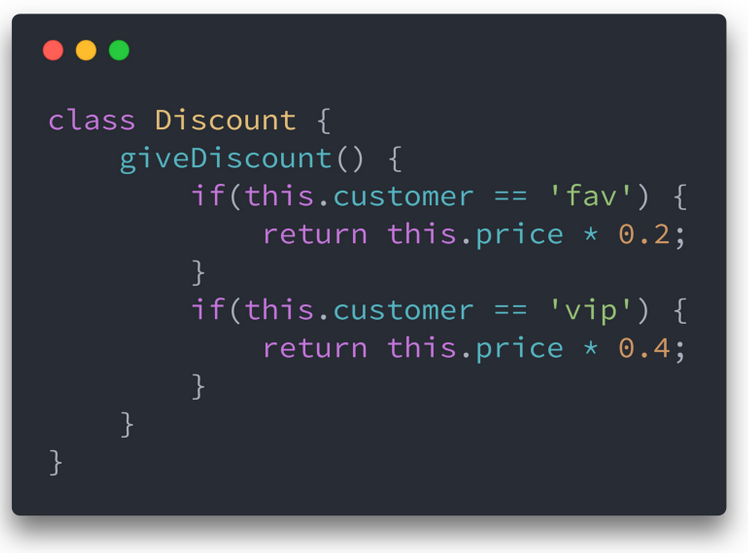
\includegraphics[scale=0.3]{l9.png}}
\end{figure}

Такой подход нарушает принцип открытости-закрытости. Как видно, здесь, если нам надо дать некоей группе клиентов особую скидку, приходится добавлять в класс новый код.

Для того чтобы переработать этот код в соответствии с принципом открытости-закрытости, добавим в проект новый класс, расширяющий класс Discount.

\newpage
В этом новом классе мы и реализуем новый механизм:

\begin{figure}[h]
\center{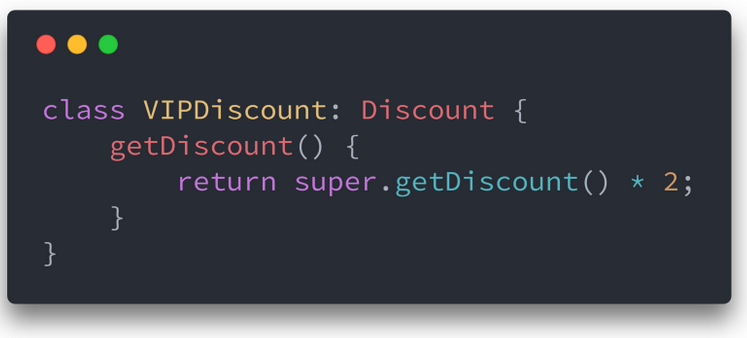
\includegraphics[scale=0.3]{l10.png}}
\end{figure}

Если решено дать скидку в 80\% «супер-VIP» клиентам, выглядеть это должно так:

\begin{figure}[h]
\center{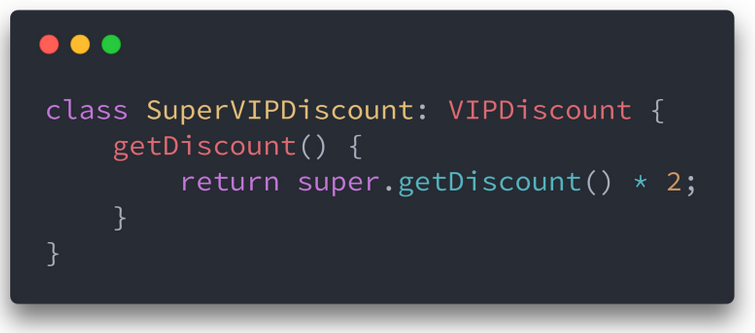
\includegraphics[scale=0.3]{l11.png}}
\end{figure}

Как видите, тут используется расширение возможностей классов, а не их модификация.

\subsection{Принцип подстановки Барбары Лисков}

\textit{Необходимо, чтобы подклассы могли бы служить заменой для своих суперклассов.}

Цель этого принципа заключаются в том, чтобы классы-наследники могли бы использоваться вместо родительских классов, от которых они образованы, не нарушая работу программы. Если оказывается, что в коде проверяется тип класса, значит принцип подстановки нарушается.

\newpage
Рассмотрим применение этого принципа, вернувшись к примеру с классом Animal. Напишем функцию, предназначенную для возврата информации о количествах конечностей животного.

\begin{figure}[h]
\center{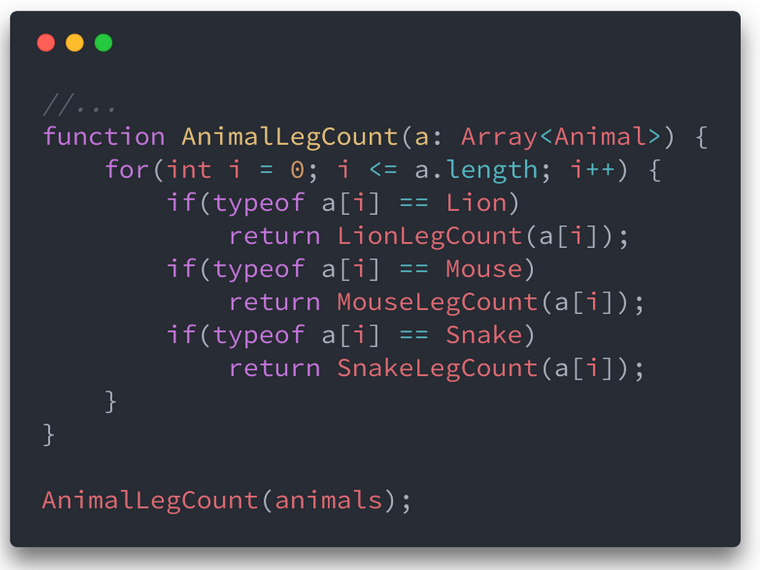
\includegraphics[scale=0.3]{l12.png}}
\end{figure}

Функция нарушает принцип подстановки (и принцип открытости-закрытости). Этот код должен знать о типах всех обрабатываемых им объектов и, в зависимости от типа, обращаться к соответствующей функции для подсчёта конечностей конкретного животного. Как результат, при создании нового типа животного функцию придётся переписывать:

\begin{figure}[h]
\center{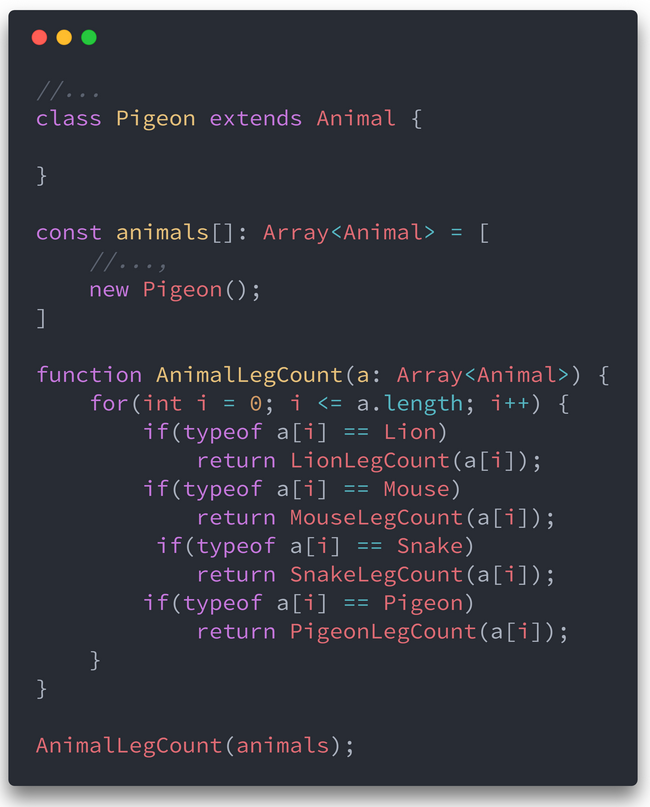
\includegraphics[scale=0.3]{l13.png}}
\end{figure}


Для того чтобы эта функция не нарушала принцип подстановки, преобразуем её с использованием требований, сформулированных Стивом Фентоном. Они заключаются в том, что методы, принимающие или возвращающие значения с типом некоего суперкласса (Animal в нашем случае) должны также принимать и возвращать значения, типами которых являются его подклассы (Pigeon).

Вооружившись этими соображениями мы можем переделать функцию AnimalLegCount:

\begin{figure}[h]
\center{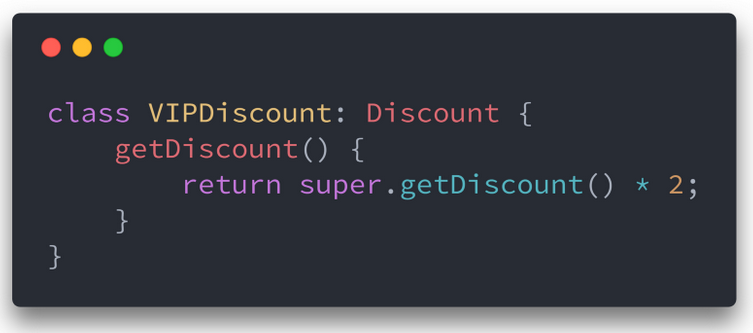
\includegraphics[scale=0.3]{l14.png}}
\end{figure}

Теперь эта функция не интересуется типами передаваемых ей объектов. Она просто вызывает их методы LegCount. Всё, что она знает о типах — это то, что обрабатываемые ей объекты должны принадлежать классу Animal или его подклассам.

Теперь в классе Animal должен появиться метод LegCount:

\begin{figure}[h]
\center{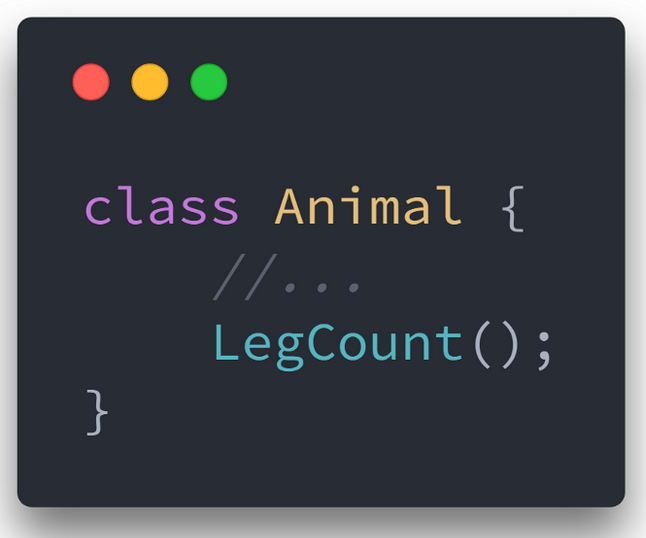
\includegraphics[scale=0.2]{l15.png}}
\end{figure}

А его подклассам нужно реализовать этот метод:

\begin{figure}[h]
\center{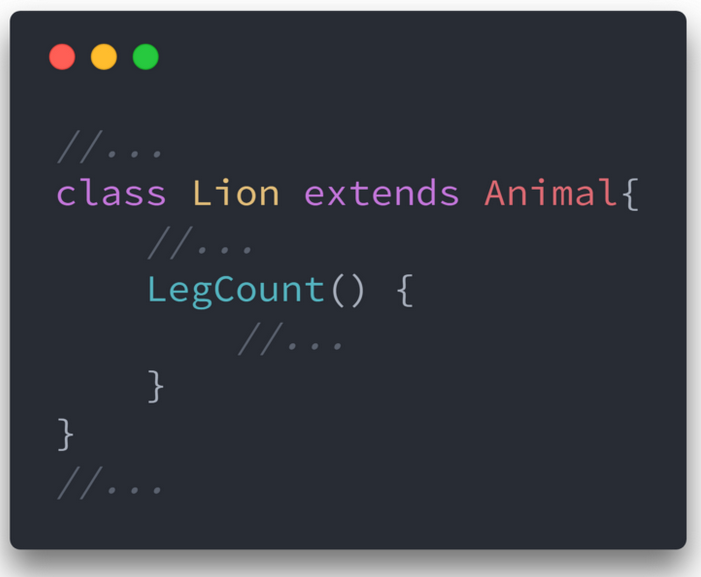
\includegraphics[scale=0.2]{l16.png}}
\end{figure}

В результате, например, при обращении к методу LegCount для экземпляра класса Lion производится вызов метода, реализованного в этом классе, и возвращается именно то, что можно ожидать от вызова подобного метода.

Теперь функции AnimalLegCount не нужно знать о том, объект какого именно подкласса класса Animalона обрабатывает для того, чтобы узнать сведения о количестве конечностей у животного, представленного этим объектом. Функция просто вызывает метод LegCount класса Animal, так как подклассы этого класса должны реализовывать этот метод для того, чтобы их можно было бы использовать вместо него, не нарушая правильность работы программы.

\subsection{Принцип разделения интерфейса}

\textit{Создавайте узкоспециализированные интерфейсы, предназначенные для конкретного клиента. Клиенты не должны зависеть от интерфейсов, которые они не используют.}

Этот принцип направлен на устранение недостатков, связанных с реализацией больших интерфейсов.

Рассмотрим интерфейс Shape:

\begin{figure}[h]
\center{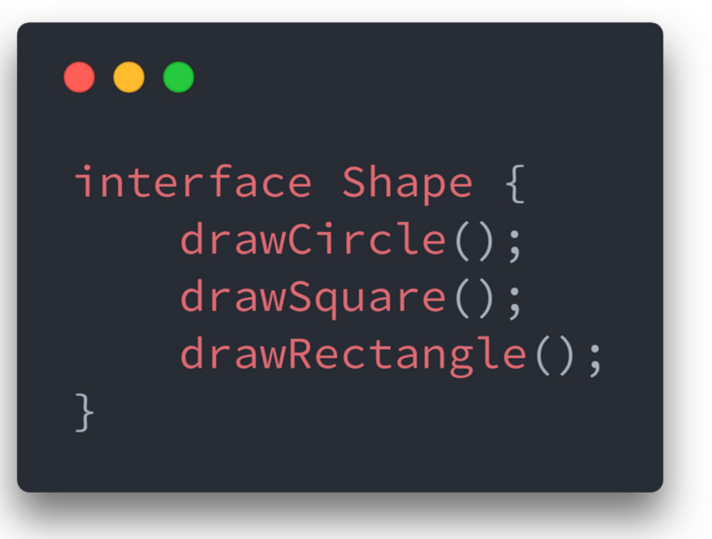
\includegraphics[scale=0.3]{l17.png}}
\end{figure}


\newpage
Он описывает методы для рисования кругов (drawCircle), квадратов (drawSquare) и прямоугольников (drawRectangle). В результате классы, реализующие этот интерфейс и представляющие отдельные геометрические фигуры, такие, как круг (Circle), квадрат (Square) и прямоугольник (Rectangle), должны содержать реализацию всех этих методов. Выглядит это так:

\begin{figure}[h]
\center{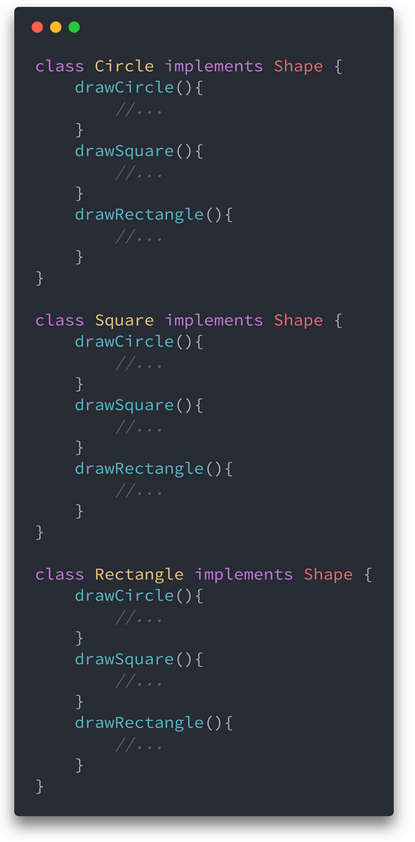
\includegraphics[scale=0.5]{l18.png}}
\end{figure}

Странный у нас получился код. Например, класс Rectangle, представляющий прямоугольник, реализует методы (drawCircle и drawSquare), которые ему совершенно не нужны. То же самое можно заметить и при анализе кода двух других классов.

\newpage
Предположим, мы решим добавить в интерфейс Shape ещё один метод, drawTriangle, предназначенный для рисования треугольников:

\begin{figure}[h]
\center{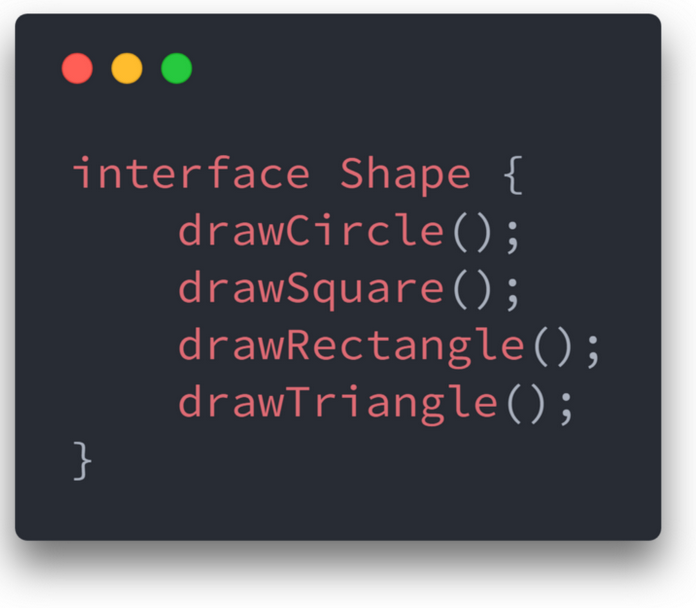
\includegraphics[scale=0.3]{l19.png}}
\end{figure}


Это приведёт к тому, что классам, представляющим конкретные геометрические фигуры, придётся реализовывать ещё и метод drawTriangle. В противном случае возникнет ошибка.

Как видно, при таком подходе невозможно создать класс, который реализует метод для вывода круга, но не реализует методы для вывода квадрата, прямоугольника и треугольника. Такие методы можно реализовать так, чтобы при их выводе выбрасывалась бы ошибка, указывающая на то, что подобную операцию выполнить невозможно.

Принцип разделения интерфейса предостерегает нас от создания интерфейсов, подобных Shape из нашего примера. Клиенты (у нас это классы Circle, Square и Rectangle) не должны реализовывать методы, которые им не нужно использовать. Кроме того, этот принцип указывает на то, что интерфейс должен решать лишь какую-то одну задачу (в этом он похож на принцип единственной ответственности), поэтому всё, что выходит за рамки этой задачи, должно быть вынесено в другой интерфейс или интерфейсы.


\newpage
В нашем же случае интерфейс Shape решает задачи, для решения которых необходимо создать отдельные интерфейсы. Следуя этой идее, переработаем код, создав отдельные интерфейсы для решения различных узкоспециализированных задач:

\begin{figure}[h]
\center{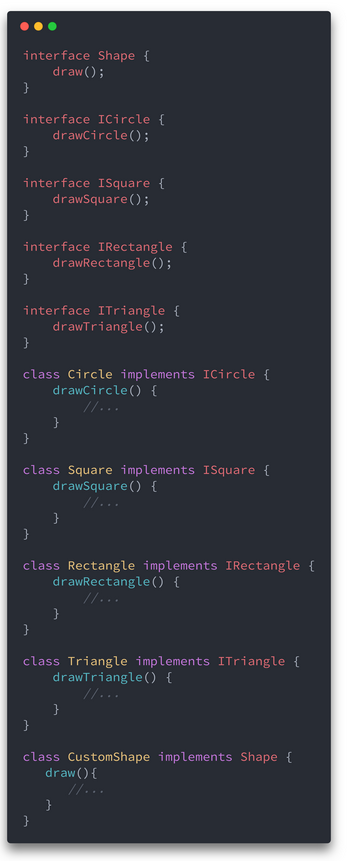
\includegraphics[scale=0.5]{l20.png}}
\end{figure}

Теперь интерфейс ICircle используется лишь для рисования кругов, равно как и другие специализированные интерфейсы — для рисования других фигур. Интерфейс Shape может применяться в качестве универсального интерфейса.

\subsection{Принцип инверсии зависимостей}

\textit{Объектом зависимости должна быть абстракция, а не что-то конкретное.}

\begin{enumerate}
  \item Модули верхних уровней не должны зависеть от модулей нижних уровней. Оба типа модулей должны зависеть от абстракций.

  \item Абстракции не должны зависеть от деталей. Детали должны зависеть от абстракций.
\end{enumerate}

В процессе разработки программного обеспечения существует момент, когда функционал приложения перестаёт помещаться в рамках одного модуля. Когда это происходит, нам приходится решать проблему зависимостей модулей. В результате, например, может оказаться так, что высокоуровневые компоненты зависят от низкоуровневых компонентов.

\begin{figure}[h]
\center{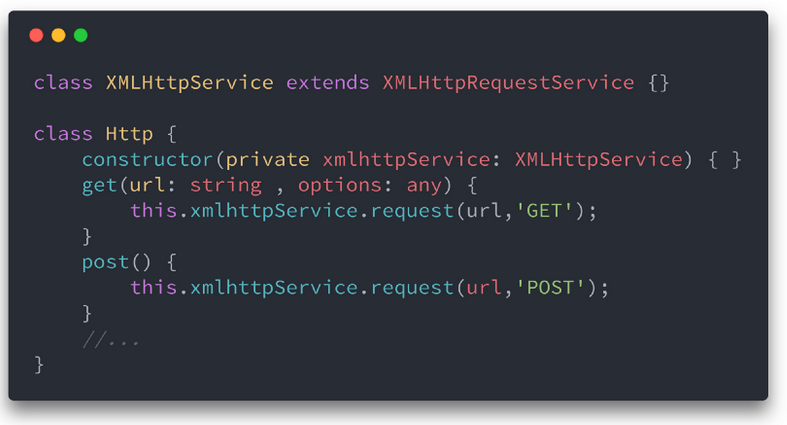
\includegraphics[scale=0.3]{l21.png}}
\end{figure}

Здесь класс Http представляет собой высокоуровневый компонент, а XMLHttpService — низкоуровневый. Такая архитектура нарушает пункт A принципа инверсии зависимостей: «Модули верхних уровней не должны зависеть от модулей нижних уровней. Оба типа модулей должны зависеть от абстракций».

Класс Http вынужденно зависит от класса XMLHttpService. Если мы решим изменить механизм, используемый классом Http для взаимодействия с сетью — скажем, это будет Node.js-сервис или, например, сервис-заглушка, применяемый для целей тестирования, нам придётся отредактировать все экземпляры класса Http, изменив соответствующий код. Это нарушает принцип открытости-закрытости.

Класс Http не должен знать о том, что именно используется для организации сетевого соединения. Поэтому мы создадим интерфейс Connection:

\begin{figure}[h]
\center{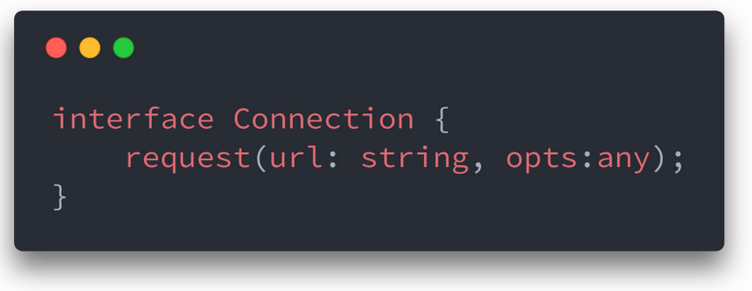
\includegraphics[scale=0.3]{l22.png}}
\end{figure}

Интерфейс Connection содержит описание метода request и мы передаём классу Http аргумент типа Connection:

\begin{figure}[h]
\center{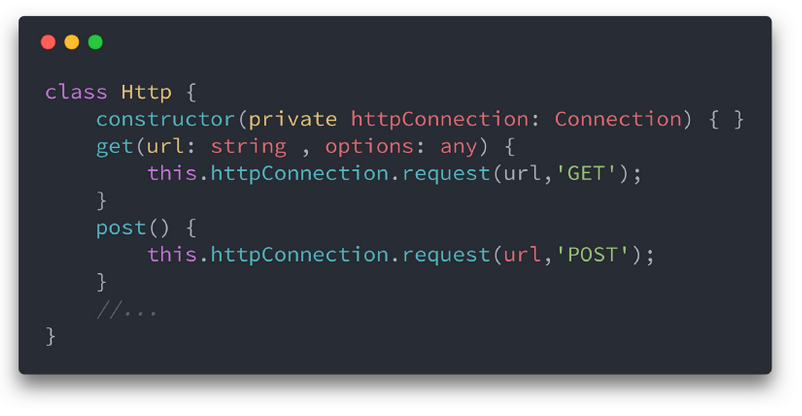
\includegraphics[scale=0.3]{l23.png}}
\end{figure}

Теперь, вне зависимости от того, что именно используется для организации взаимодействия с сетью, класс Http может пользоваться тем, что ему передали, не заботясь о том, что скрывается за интерфейсом Connection.

Перепишем класс XMLHttpService таким образом, чтобы он реализовывал этот интерфейс:

\begin{figure}[h]
\center{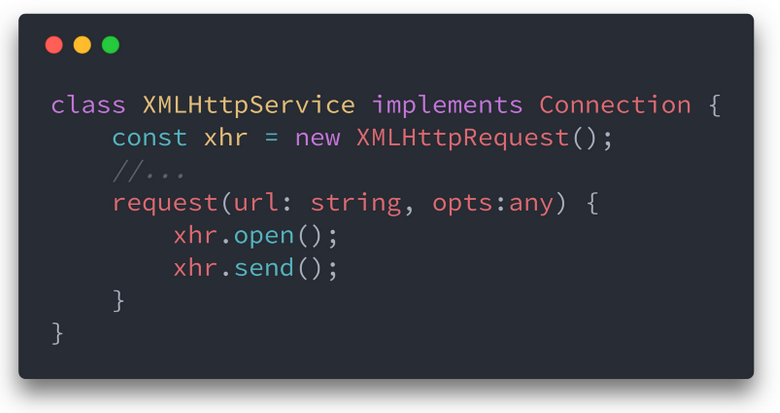
\includegraphics[scale=0.3]{l24.png}}
\end{figure}

В результате мы можем создать множество классов, реализующих интерфейс Connection и подходящих для использования в классе Http для организации обмена
данными по сети:

\begin{figure}[h]
\center{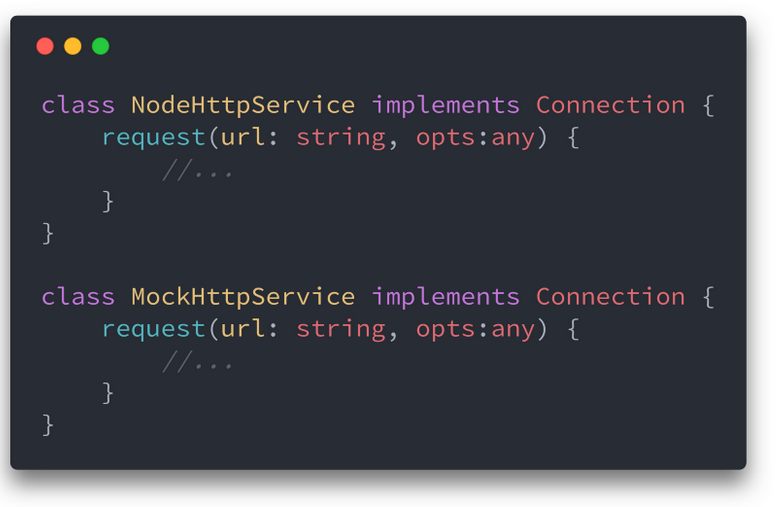
\includegraphics[scale=0.3]{l25.png}}
\end{figure}

Как можно заметить, здесь высокоуровневые и низкоуровневые модули зависят от абстракций. Класс Http (высокоуровневый модуль) зависит от интерфейса Connection (абстракция). Классы XMLHttpService, NodeHttpService и MockHttpService (низкоуровневые модули) также зависят от интерфейса Connection.

Кроме того, стоит отметить, что следуя принципу инверсии зависимостей, мы соблюдаем и принцип подстановки Барбары Лисков. А именно, оказывается, что типы XMLHttpService, NodeHttpService и MockHttpService могут служить заменой базовому типу Connection.

\textbf{Итоги}

Здесь мы рассмотрели пять принципов SOLID, которых следует придерживаться каждому ООП-разработчику. Поначалу это может оказаться непросто, но если к этому стремиться, подкрепляя желания практикой, данные принципы становятся естественной частью рабочего процесса, что оказывает огромное положительное воздействие на качество приложений и значительно облегчает их поддержку.

\section{Антипаттерны}

\section{Continuous integration}

\section{Методология разработки ПО}

У любого программного обеспечения есть жизненный цикл — этапы, через которые оно проходит с начала создания до конца разработки и внедрения. Чаще всего это подготовка, проектирование, создание и поддержка. Этапы могут называться по-разному и дробиться на более мелкие стадии.

\begin{figure}[h]
\center{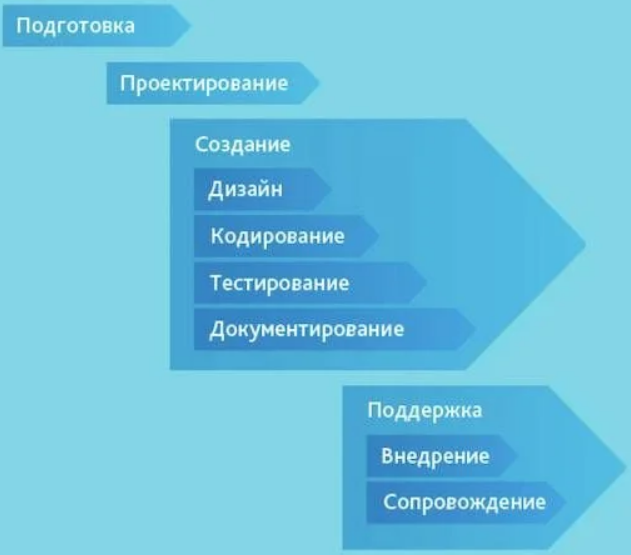
\includegraphics[width=\textwidth]{m1.png}}
\end{figure}

Рассмотрим эти этапы на примере жизненного цикла интернет-магазина.

\noindent\textbf{Подготовка.} Вы решили запустить книжный интернет-магазин и начали анализировать, какие подобные сайты уже представлены в сети. Собрали информацию об их трафике, функциональности.

\noindent\textbf{Проектирование.} Вы выбрали компанию-подрядчика и обсудили с её специалистами архитектуру и дизайн будущего интернет-магазина.

\noindent\textbf{Создание.} Вы заключили с разработчиками договор. Они начали писать код, отрисовывать дизайн, составлять документацию.

\noindent\textbf{Поддержка.} Вы подписали акт сдачи-приёмки, и подрядчик разместил интернет-магазин на «боевых» серверах. Пользователи начали его посещать и сообщать о замеченных ошибках в поддержку, а программисты — оперативно всё исправлять.

\noindent\textit{Модель} разработки программного обеспечения описывает, какие стадии жизненного цикла оно проходит и что происходит на каждой из них.

\noindentА \textit{методология} включает в себя набор методов по управлению разработкой: это правила, техники и принципы, которые делают её более эффективной.

\subsection{Основные модели разработки ПО}

\begin{itemize}
    \item Code and fix — модель кодирования и устранения ошибок;
    \item Waterfall Model — каскадная модель, или «водопад»;
    \item V-model — V-образная модель, разработка через тестирование;
    \item Incremental Model — инкрементная модель;
    \item Iterative Model — итеративная (или итерационная) модель;
    \item Spiral Model — спиральная модель;
    \item Chaos model — модель хаоса;
    \item Prototype Model — прототипная модель.
\end{itemize}

Из этих моделей наиболее популярны пять основных: каскадная, V-образная, инкрементная, итерационная и спиральная. Разберём их подробнее.

\subsubsection{Waterfall (каскадная модель, или «водопад»)}

В этой модели разработка осуществляется поэтапно: каждая следующая стадия начинается только после того, как заканчивается предыдущая. Если всё делать правильно, «водопад» будет наиболее быстрой и простой моделью. Применяется уже почти полвека, с 1970-х.


\begin{figure}[h]
\center{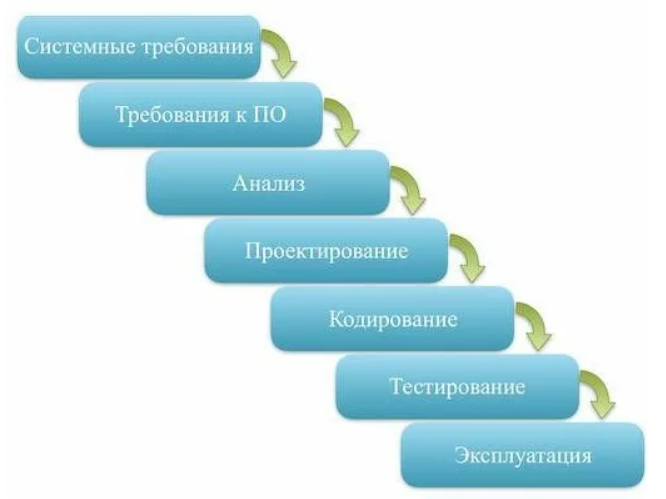
\includegraphics[width=\textwidth]{m2.png}}
\end{figure}

\noindent\textbf{Преимущества «водопада»}

\begin{itemize}
    \item Разработку просто контролировать. Заказчик всегда знает, чем сейчас заняты программисты, может управлять сроками и стоимостью.
    \item Стоимость проекта определяется на начальном этапе. Все шаги запланированы уже на этапе согласования договора, ПО пишется непрерывно «от и до».
    \item Не нужно нанимать тестировщиков с серьёзной технической подготовкой. Тестировщики смогут опираться на подробную техническую документацию.
\end{itemize}

\noindent\textbf{Недостатки каскадной модели}

\begin{itemize}
    \item     Тестирование начинается на последних этапах разработки. Если в требованиях к продукту была допущена ошибка, то исправить её будет стоить дорого. Тестировщики обнаружат её, когда разработчик уже написал код, а технические писатели — документацию.
    \item Заказчик видит готовый продукт в конце разработки и только тогда может дать обратную связь. Велика вероятность, что результат его не устроит.
    \item Разработчики пишут много технической документации, что задерживает работы. Чем обширнее документация у проекта, тем больше изменений нужно вносить и дольше их согласовывать.
\end{itemize}

«Водопад» подходит для разработки проектов в медицинской и космической отрасли, где уже сформирована обширная база документов (СНиПов и спецификаций), на основе которых можно написать требования к новому ПО.

При работе с каскадной моделью основная задача — написать подробные требования к разработке. На этапе тестирования не должно выясниться, что в них есть ошибка, которая влияет на весь продукт.

\subsubsection{V-образная модель (разработка через тестирование)}

Это усовершенствованная каскадная модель, в которой заказчик с командой программистов одновременно составляют требования к системе и описывают, как будут тестировать её на каждом этапе. История этой модели начинается в 1980-х.


\begin{figure}[h]
\center{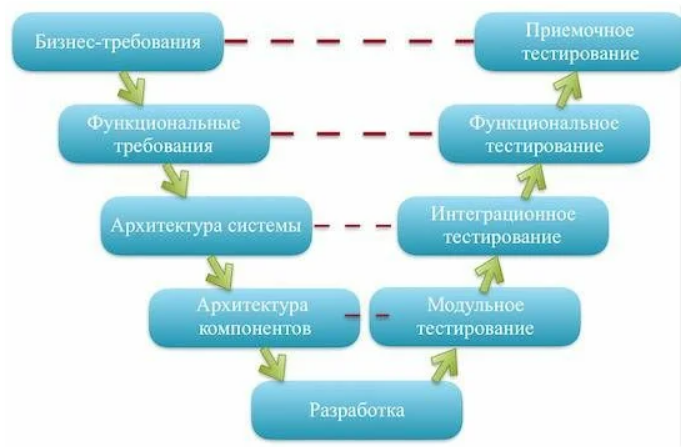
\includegraphics[width=\textwidth]{m3.png}}
\end{figure}

\noindent\textbf{Преимущества V-образной модели}
\begin{itemize}
  \itemКоличество ошибок в архитектуре ПО сводится к минимуму.
\end{itemize}
\noindent\textbf{Недостатки V-образной модели}
\begin{itemize}
  \item Если при разработке архитектуры была допущена ошибка, то вернуться и исправить её будет стоить дорого, как и в «водопаде».
\end{itemize}

V-модель подходит для проектов, в которых важна надёжность и цена ошибки очень высока. Например, при разработке подушек безопасности для автомобилей или систем наблюдения за пациентами в клиниках.

\subsubsection{Incremental Model (инкрементная модель)}

Это модель разработки по частям (increment в переводе с англ. — приращение) уходит корнями в 1930-е. Рассмотрим её на примере создания социальной сети.

\begin{itemize}
    \item Заказчик решил, что хочет запустить соцсеть, и написал подробное техническое задание. Программисты предложили реализовать основные функции — страницу с личной информацией и чат. А затем протестировать на пользователях, «взлетит или нет».
    \item Команда разработки показывает продукт заказчику и выпускает его на рынок. Если и заказчику, и пользователям социальная сеть нравится, работа над ней продолжается, но уже по частям.
    \item Программисты параллельно создают функциональность для загрузки фотографий, обмена документами, прослушивания музыки и других действий, согласованных с заказчиком. Инкремент за инкрементом они совершенствуют продукт, приближаясь к описанному в техническом задании.
\end{itemize}

\begin{figure}[h]
\center{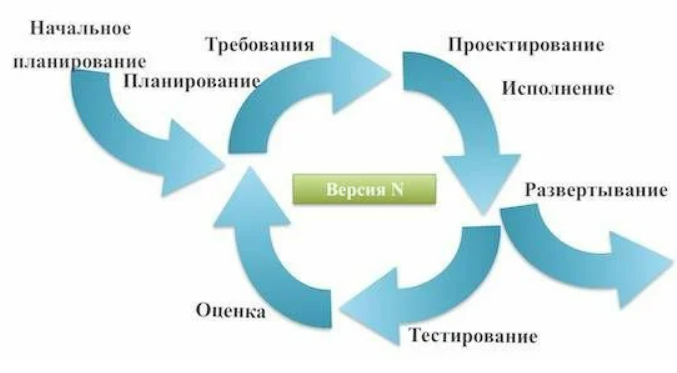
\includegraphics[width=\textwidth]{m4.png}}
\end{figure}

\noindent\textbf{Преимущества инкрементной модели}
\begin{itemize}
  \item    Не нужно вкладывать много денег на начальном этапе. Заказчик оплачивает создание основных функций, получает продукт, «выкатывает» его на рынок — и по итогам обратной связи решает, продолжать ли разработку.
  \item Можно быстро получить фидбэк от пользователей и оперативно обновить техническое задание. Так снижается риск создать продукт, который никому не нужен.
  \item Ошибка обходится дешевле. Если при разработке архитектуры была допущена ошибка, то исправить её будет стоить не так дорого, как в «водопаде» или V-образной модели.
\end{itemize}
\noindent\textbf{Недостатки инкрементной модели}
\begin{itemize}
  \item Каждая команда программистов разрабатывает свою функциональность и может реализовать интерфейс продукта по-своему. Чтобы этого не произошло, важно на этапе обсуждения техзадания объяснить, каким он будет, чтобы у всех участников проекта сложилось единое понимание.
  \item Разработчики будут оттягивать доработку основной функциональности и «пилить мелочёвку». Чтобы этого не случилось, менеджер проекта должен контролировать, чем занимается каждая команда.
\end{itemize}

Инкрементная модель подходит для проектов, в которых точное техзадание прописано уже на старте, а продукт должен быстро выйти на рынок.

\subsubsection{Iterative Model (итеративная модель)}

Это модель, при которой заказчик не обязан понимать, какой продукт хочет получить в итоге, и может не прописывать сразу подробное техзадание.

\begin{figure}[h]
\center{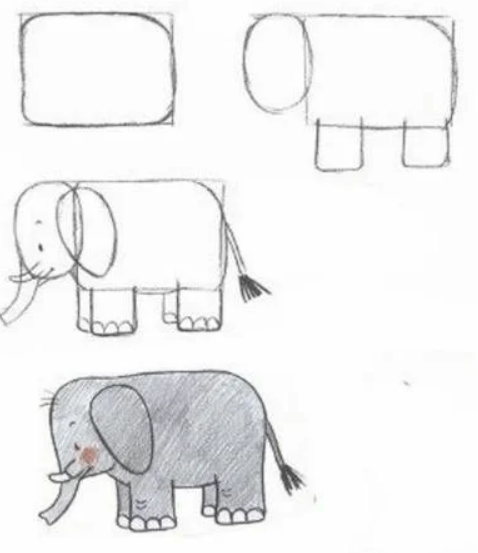
\includegraphics[width=\textwidth]{m5.png}}
\end{figure}

Рассмотрим на примере создания мессенджера, как эта модель работает.
\begin{itemize}
    \item Заказчик решил, что хочет создать мессенджер. Разработчики сделали приложение, в котором можно добавить друга и запустить чат на двоих.
    \item Мессенджер «выкатили» в магазин приложений, пользователи начали его скачивать и активно использовать. Заказчик понял, что продукт пользуется популярностью, и решил его доработать.
    \item Программисты добавили в мессенджер возможность просмотра видео, загрузки фотографий, записи аудиосообщений. Они постепенно улучшают функциональность приложения, адаптируют его к требованиям рынка.
\end{itemize}

\noindent\textbf{Преимущества итеративной модели}
\begin{itemize}
  \item Быстрый выпуск минимального продукта даёт возможность оперативно получать обратную связь от заказчика и пользователей. А значит, фокусироваться на наиболее важных функциях ПО и улучшать их в соответствии с требованиями рынка и пожеланиями клиента.
  \item Постоянное тестирование пользователями позволяет быстро обнаруживать и устранять ошибки.
\end{itemize}

\noindent\textbf{Недостатки итеративной модели}
\begin{itemize}
  \item Использование на начальном этапе баз данных или серверов — первые сложно масштабировать, а вторые не выдерживают нагрузку. Возможно, придётся переписывать большую часть приложения.
  \item Отсутствие фиксированного бюджета и сроков. Заказчик не знает, как выглядит конечная цель и когда закончится разработка.
\end{itemize}

Итеративная модель подходит для работы над большими проектами с неопределёнными требованиями, либо для задач с инновационным подходом, когда заказчик не уверен в результате.

\subsubsection{Spiral Model (спиральная модель)}

Используя эту модель, заказчик и команда разработчиков серьёзно анализируют риски проекта и выполняют его итерациями. Последующая стадия основывается на предыдущей, а в конце каждого витка — цикла итераций — принимается решение, продолжать ли проект. Эту модель начали использовать в 1988 году.

\begin{figure}[h]
\center{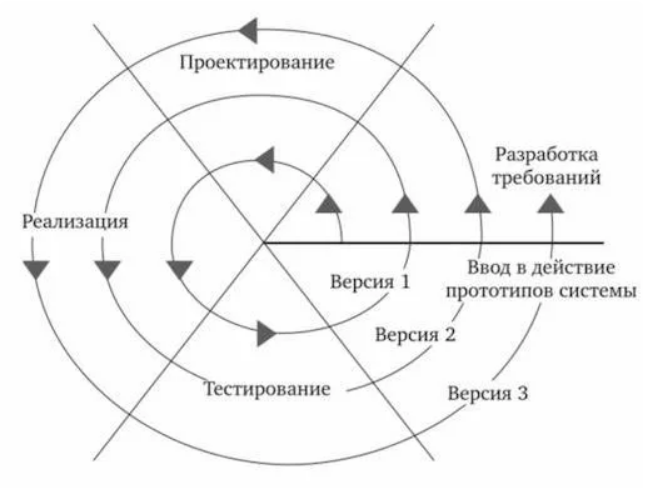
\includegraphics[width=\textwidth]{m6.png}}
\end{figure}

Рассмотрим, как функционирует эта модель, на примере разработки системы «Умный дом».
\begin{itemize}
    \item Заказчик решил, что хочет сделать такую систему, и заказал программистам реализовать управление чайником с телефона. Они начали действовать по модели «водопад»: выслушали идею, провели анализ предложений на рынке, обсудили с заказчиком архитектуру системы, решили, как будут её реализовывать, разработали, протестировали и «выкатили» конечный продукт.
    \item Заказчик оценил результат и риски: насколько нужна пользователям следующая версия продукта — уже с управлением телевизором. Рассчитал сроки, бюджет и заказал разработку. Программисты действовали по каскадной модели и представили заказчику более сложный продукт, разработанный на базе первого.
    \item Заказчик подумал, что пора создать функциональность для управления холодильником с телефона. Но, анализируя риски, понял, что в холодильник сложно встроить Wi-Fi-модуль, да и производители не заинтересованы в сотрудничестве по этому вопросу. Следовательно, риски превышают потенциальную выгоду. На основе полученных данных заказчик решил прекратить разработку и совершенствовать имеющуюся функциональность, чтобы со временем понять, как развивать систему «Умный дом».
\end{itemize}


Спиральная модель похожа на инкрементную, но здесь гораздо больше времени уделяется оценке рисков. С каждым новым витком спирали процесс усложняется. Эта модель часто используется в исследовательских проектах и там, где высоки риски.

\noindent\textbf{Преимущества спиральной модели}
\begin{itemize}
  \item Большое внимание уделяется проработке рисков.
\end{itemize}
\noindent\textbf{Недостатки спиральной модели}
\begin{itemize}
  \item Есть риск застрять на начальном этапе — бесконечно совершенствовать первую версию продукта и не продвинуться к следующим.
  \item Разработка длится долго и стоит дорого.
\end{itemize}

На основе итеративной модели была создана Agile — не модель и не методология, а скорее подход к разработке.

\subsection{Agile}

Agile («эджайл») переводится с английского как «гибкий». Включает в себя практики, подходы и методологии, которые помогают создавать продукт более эффективно:

\begin{itemize}
    \item экстремальное программирование (Extreme Programming, XP);
    \item бережливую разработку программного обеспечения (Lean);
    \item фреймворк для управления проектами Scrum;
    \item разработку, управляемую функциональностью (Feature-driven development, FDD);
    \item разработку через тестирование (Test-driven development, TDD);
    \item методологию «чистой комнаты» (Cleanroom Software Engineering);
    \item итеративно-инкрементальный метод разработки (OpenUP);
    \item методологию разработки Microsoft Solutions Framework (MSF);
    \item метод разработки динамических систем (Dynamic Systems Development Method, DSDM);
    \item метод управления разработкой Kanban.
\end{itemize}

Не всё перечисленное в списке — методологии. Например, Scrum чаще называют не методологией, а фреймворком. В чём разница? Фреймворк — это более сформированная методология со строгими правилами. В скраме все роли и процессы чётко прописаны. Помимо Scrum, часто используют Kanban.

\end{document}
